\documentclass{l3proj}

\title{A Hands-on Approach to Learning Molecular Biology Techniques}
\author{
  Ross Eric Barnie \\
  Dmitrijs Jonins \\
  Daniel McElroy \\
  Murray Ross \\
  Ross Taylor
}
\date{18th March 2013}

\usepackage{mystyle}

\begin{document}
\maketitle
\begin{abstract}

Abstract-like things

\end{abstract}
\centerline{Acknowledgements}

First of all, we would like to thank our supervisor, Dr Gethin Norman, for his guidance, organisational skills and support throughout this project. We would also like to thank Dr Nicola Veitch and Dr Pamela Scott for their assistance with all matters relating to PCR and Primer design.

\educationalconsent
\tableofcontents

%=====================================================================
\chapter{Introduction}
\label{intro}

\section{Preliminaries}
\label{intro:prelims}
% Need to explain NCBI, BLAST

There are some terms that will be used later in the report that should
be clarified here, so as to avoid confusion.
The aim of the project is to creating a teaching tool for PCR, or
Polymerase Chain Reactions.
This is the process of amplifying a specified sequence of DNA thousands to
millions of times.
It should be explained that DNA sequences are made up of two strands,
comprised of bases of the nucleotides Adenine, Thymine, Guanine and
Cytosine, represented by the letters \verb£a£, \verb£t£, \verb£g£, and
\verb£c£ respectively.
Base pairing is when one base bonds with its complement on the other
strand.
The bases \verb£a£ and \verb£t£ complement each other, and bases
\verb£g£ and \verb£c£ complement each other.

Primers, used to select the sequence for PCR in a given selection of
DNA, are shorter fragments of DNA, usually between 20 and 30 bases in
length.
For use in PCR, a primer must be chosen from the ``left'' of one
strand (this is the forward primer) and the ``right'' of the other
(this is the reverse primer), and these must obey a number of rules,
which are the focus of the teaching tool:
\begin{itemize}
\item Neither primer should self-anneal. 
  This means that if the primer were to fold over
  in such a way that that more than 3 bases in a row on one side
  complemented the bases on the opposite side, this primer would pair 
  with itself and become useless for the purposes of PCR.
\item The melting temperature of each primer, calculated in degrees
  Celsius using a simple mathematical formula involving the frequency
  of \verb£a£s, \verb£t£s, \verb£g£s and \verb£c£s, should be between
  50 and 65\degree C, and within 2-3\degree C of each other.
\item The forward primer should be unique within the first strand, and
  not appear in the second, complementary strand. Likewise, the
  reverse primer should be unique within the second strand and should
  not appear in the first.
\item The percentage of \verb£g£s and \verb£c£s within each primer
  should be between 40\% and 60\%.
\item The length of each primer should be between 20 and 30 bases.
\item The same base should not be repeated several times in a row in
  either primer.
\item The last base of each primer should be either a \verb£g£ or a
  \verb£c£.
\item The primers should not anneal to each other. 
  This means that if the primers were put side by side, at no point of
  overlap should more than 3 bases in a row complement the overlapping
  primer’s base.
\end{itemize}

It should be noted that many of these rules are not precise, and do
not involve rigid limits for success or failure.
In fact, these ``rules'' more closely resemble rough guides.
Obviously, the nature of programming does not lend itself to ``rough
guides'', and so we followed advice from Pamela Scott and Nicola
Veitch on how best to structure these tests to effectively represent
the imprecision of their boundaries.

The ends of strands of DNA are often referred to as the ``5'-end'' and
the ``3'end'' which are named as such due to the positioning of carbon
atoms near to the ends of the strand. This naming convention allows DNA
strand orientation to be described as either ``5'-3''' or ``3'-5'''.
This is relevant to PCR and primer design because strands anneal to
each other by the 5'-ends of the strands joining to the 3'-ends of the
other strand.

\begin{figure}[!t]
  \begin{center}
    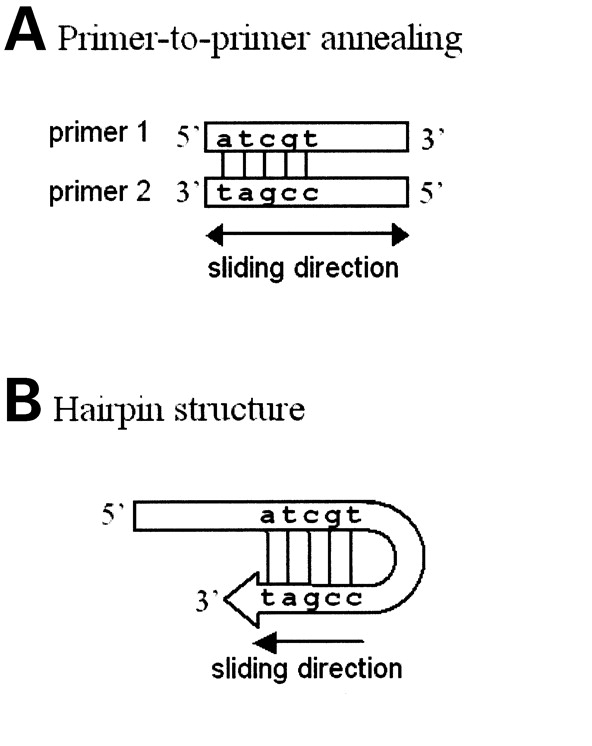
\includegraphics[width=0.75\textwidth]{./images/other/annealing.jpg}
    \caption{
      \label{fig:other:anneal}
      Annealing	
    }
  \end{center}
\end{figure}








%--------------------------------------------------------------------------

Two external services that are integral to the successful use of the system
are the National Center for Biotechnology Information (NCBI) \cite{ncbi},
and the use of a Basic Local Alignment Search Tool. NCBI is, for the purposes
of this exercise, a vast database of DNA sequences and related information,
from which the user can obtain a sequence on which to perform PCR (though this
can also be obtained from other sources). At the end of the exercise, the
user is encouraged to use the BLAST functionality on the NCBI website to ensure
that their primer is specific to their intended PCR target.

It should also be explained that we developed the teaching tool
in Java, using Netbeans, a free IDE primarily designed to be used with
Java, and developing the user interface with Swing, the primary Java 6
GUI framework and that we stored all project-related files in a
version-controlled repository hosted by GitHub.



\section{Aims}
\label{intro:aims}
The overall aim of this project is to produce a piece of software to
help Level 3 Life Sciences students taking the Molecular Methods
course (taught by Drs. Pamela Scott and Nicola Veitch) learn about PCR
and Primer Design Techniques and to allow them to test their knowledge
of these subjects. At the outset of the project, Scott and Veitch
helped us to separate this aim into key tasks to be completed and
important aspects of the interface design to be implemented:

\begin {enumerate}

\item The software should work as an interactive tutorial which users
  can work through. This requires:

\begin {itemize}
\item A number of areas for users to enter their own choice of data,
  such as a choice of DNA sequence to work with and the primers with
  which to operate on the selected strand. For this feature to be
  useful as an educational tool feedback must be provided upon data
  entry.
\item Users should be able to experiment with different data
  e.g. examining the different melting temperatures of different
  primers. This requires the ability to easily move forwards and
  backwards between the different stages of the tutorial.
\item To help newer users and students who are unfamiliar with PCR
  there should be simple instructions to guide users through the
  process and explain PCR throughout the application. The user 
  should also be able to access the rules of PCR and primer design 
  at any time.
\end {itemize}

\item The software should be accessible to all users with a basic
  understanding of molecular biology, regardless of their different
  levels of knowledge, ability etc.:

\begin {itemize}
\item To achieve this, the interface should be uncomplicated and
  intuitive without compromising the required functionality. This will
  be aided by the instructions and help section mentioned above, as
  well as labels placed next to any areas users can interact with.
\item Any section which makes use of colour should be designed with
  colour blind users in mind.
\end {itemize}

\item The software should improve upon the tools currently available
  for learning primer design. The main issues with these systems are: 

\begin {itemize}
\item The low level of interactivity offered by the systems, such as
  the numerous YouTube videos available on the subject
  \cite{youtube:taqExtension}. Users who are not actively working
  through a tutorial or a demonstration are likely to lose interest
  faster so it is important to make them involved with every step of
  the tutorial by having them design their own primers etc.
\item The available tools rarely go into detail about primer design
  specifically. One example of an interactive, well designed
  application that fails to convey the process of designing primers to
  a satisfactory degree is University of Utah's "PCR Virtual Lab"
  \cite{genScienceCenter2012}. Therefore, an important aim for the
  project is that primer design must be explained in detail and
  provide enough information to be informative, whilst remaining
  interesting to students using the system.
\end {itemize}

\item Another aim related to accessibility is that the users should be
  able to download and use the software from home. This means that the
  program must be able to run on a variety of different operating
  systems and computers with varying performance levels. With this in
  mind it was decided that the program should be written in Java due
  to it being highly portable.
\end {enumerate}


\section{Background}
\label{intro:background}

\section{Motivation}
\label{intro:motiv}
At the beginning of the project we were sent three links to systems
currently in place which attempt to make learning this process more
interactive and/or visual.

The first was a video hosted on YouTube \citep{youtube:taqExtension},
made by demonstrators within the School of Life Sciences.
During its eighteen second duration, the video shows various elements
of the PCR process including change in temperature and the role of the
primer.
However, it was commented by the team and by the clients that it was
insubstantial in terms of information delivery, several of the stages
of PCR are omitted with no mention of primer design, and in terms
of interactivity.

Another video hosted on YouTube \citep{youtube:PCR}, currently referred
to on School of Life Sciences' website, is similar in style to a
lecture with slides and a voice-over which repeats the textual
information on each slide.
While this video is far more informative than the previous one, with
each stage of PCR clearly described, and with visually pleasing
animations, it lacks in explicit primer design and again in
interactivity.

Videos and multimedia in general have been questioned as teaching
aids.
Simply because the information is in video or multimedia format
does not necessarily mean that it is benefitting the learning of its
viewers, or creating the correct environment to encourage learning.
Interactivity, along with other factors, are key to engaging people to
learn \citep{gamingRedefines2004}.

Finally, an animation from the University of Utah, titled ``PCR
Virtual Lab'' \citep{genScienceCenter2012}.
This is a much more interactive experience and allows the user to use
virtual pipettes in order to simulate what you would do in a lab
situation when performing PCR.
Additionally, the information it provides, while slightly basic in the
beginning for our target users, is extensive and very informative to
the novice user, such as Biology-illiterate Computing Scientists.
While this is a much more interactive and, compared to the
alternatives described above, much more informative experience, it
fails to provide the user with the theoretical background information,
particularly on primer design, required to fully understand the
process and why the reaction occurs.


%=====================================================================
\chapter{Design}
\label{design}

\section{Requirements}
\label{design:reqs}
% WILL NEED THE FOLLOWING:
% FIGURES - original meeting notes - FIND THEM
%         - Dmitrijs' designs, and any others we can find

\subsubsection{Inital Requirements Gathering}
% The sheet we were presented with Meeting 1 - flow of application more 
% or less already decided
% Molecular Methods lab book
% Links to Youtube videos and Utah thang
The requirements gathering process for the application began immediately.
At the first meeting, our clients presented us with a document outlining
what it was that they wanted from the end product, including a very
early step-by-step walkthrough of the application they envisioned. This
proved to be a key tool in bringing us up to speed with what the system
should accomplish, and really sped up the initial requirements gathering
phase. This design was altered and adapted throughout the
project, but the steps served to provide a rough guidline that we
followed throughout development. The aim of the project, as described in
the aforementioned document, are as follows:
\begin{quotation}
To design a PCR-primer design exercise to complement teaching of a
Molecular Methods course to Level 3 Life Sciences Undergraduates. This
exercise will be integrated into a new part of the lab which we are
designing based around diagnosis of HIV using PCR. You will need to
understand the theory behind PCR and primer design in order to achieve
this.
\end{quotation}
This statement alone is helpful as it tells us about our userbase, where
and how the application will be used, and what background knowledge is
required in order to thoroughly understand the premise of the project.

On the subject of background knowledge, along with this document, we 
were given the Molecular Methods lab book, in order to see how Primer 
Design is currently taught in the course and get a better idea of how
it worked ourselves.
% TALK ABOUT MOL METHODS BOOK, WHAT COULD BE IMPROVED.
%---------------------------------------------------------------------------------------------DON'T FORGET ABOUT THIS BROSSOLINI

Finally, within the first two or three meetings we were sent links to
various multimedia teaching tools for Primer Design, as described in
Section \ref{intro:currentSystems}. Along with our own research, this
gave us an informed view of the current climate of PCR teaching tools,
the positives and negatives of these current approaches, and what we
could improve upon in our own product.

From these first few weeks of meetings with the clients, we drafted a
requirements document, which was presented to the clients and agreed upon,
and presented the following requirements:

\paragraph{System Scope}
\begin{itemize}
\item{The main aim of this system is to act as a teaching tool to aid 
students in learning how to design primers for PCR experiments and 
should be usable in a teaching environment or by people on their home 
computers.}
\item{It should function as an interactive, step-by-step guide through 
the process of PCR on a DNA strand of the user's choice. The user is 
required to access the NCBI website \cite{ncbi} and copy and paste
their choice of DNA sequence into the system.
The system should provide feedback if the user enters incorrect
primers.
The system should then check if the melting temperatures of the
primers are in the required range, using the equation provided to us
by the clients. This equation should be visible to the user.
The user is then given a link to perform primer BLAST (described in 
Section \ref{intro:prelims})
to check if the primers they have chosen are unique.}
\item{The system should also provide the user help with completing each 
task by providing relevant rules for each task and giving the user 
instructions about how to use websites and resources outwith the system 
(NCBI \cite{ncbi}, primer BLAST \cite{blast} etc.).}
\item{When the user has provided an appropriate pair of primers the 
system will then show an animation of the PCR reaction taking place.}
\end{itemize}
\paragraph{Non-Functional Requirements}
\begin{itemize}
\item{The system is expected to be used at students’ homes or in the 
Biology lab computers, so portability is essential for the system to 
work to the clients’ expectations.}
\end{itemize}

We found that while several aspects of the system deviated from the
document we were handed in the first meeting, the requirements largely
stayed the same throughout.

\subsubsection{Design Feedback}
% Produced several versions of user interface mockups
Throughout the project, we maintained a weekly meeting schedule with our
supervisor and clients, and despite scheduling difficulties at least one
of the clients was present at every one of these meetings. This allowed
us the opportunity to improve our design iteratively through multiple
pitches, internalising the feedback given over the following week to 
produce a design more in line with their requirements.

When the team had formed a solid idea of the layout and flow of the
system, we drew up some early mockups of the system's user interface
(discussed in further detail in Section \ref{design:ui}) and presented
them to the clients during 
one of the weekly meetings %DATE IF POSSIBLE
to get their feedback on the design and how they felt it met the 
requirements. 

We asked a number of questions related to both the user
interface and our understanding of PCR, and found that they were largely
satisfied with prototype design. This prototype did not feature the
animation described in the requirements, but we received valuable feedback
on the validity of the system described by the prototype as a teaching
tool.


\subsubsection{Implementation Feedback}
% At weekly meetings during implementation, gave repeated demonstrations
% Clients were always more than happy to provide a number of suggestions
% and improvements in keeping with the requirements of the product.
Once implementation was fully underway and the application had reached
a demonstrable state, we began presenting our progress at the weekly client
meetings. We received substantial feedback on how to change the UI and 
how the primer checks were handled in order
to best improve the product as a teaching tool, and to be as accurate to
the primer design process as possible.  


\section{UI}
\label{design:ui}
The User Interface design was developed based on the feedback and guidelines set by the clients, the Biology department staff. As it was an abstraction, we decided developing it in Microsoft Power Point was adequate for flexibility of the deisgn document and provides sufficient tools to make it presentable. Four main stages of the UI were separated into five slides which are provided and explained below.


\subsubsection{Sequence entry}
The first slide shows the sequence entry screen, where the user copies the DNA sequence on which to perform PCR into the provided box. The backward DNA strand is calculated right away and shown in green text, with each line being a complementary sequence of the one above. The numbers on the left show the node number at the start of the corresponding line. It is a way for the user to quickly find the part of the sequence to be amplified in the next stage and to provide better orientation in the sequence altogether. Scrolling through the sequence is done by pressing the arrow buttons on the right or just using the scroll wheel of the mouse. Once the user is content with the sequence entered, he can press the "Go" button to advance to the next stage.

\begin{figure}[h]
  \begin{center}
	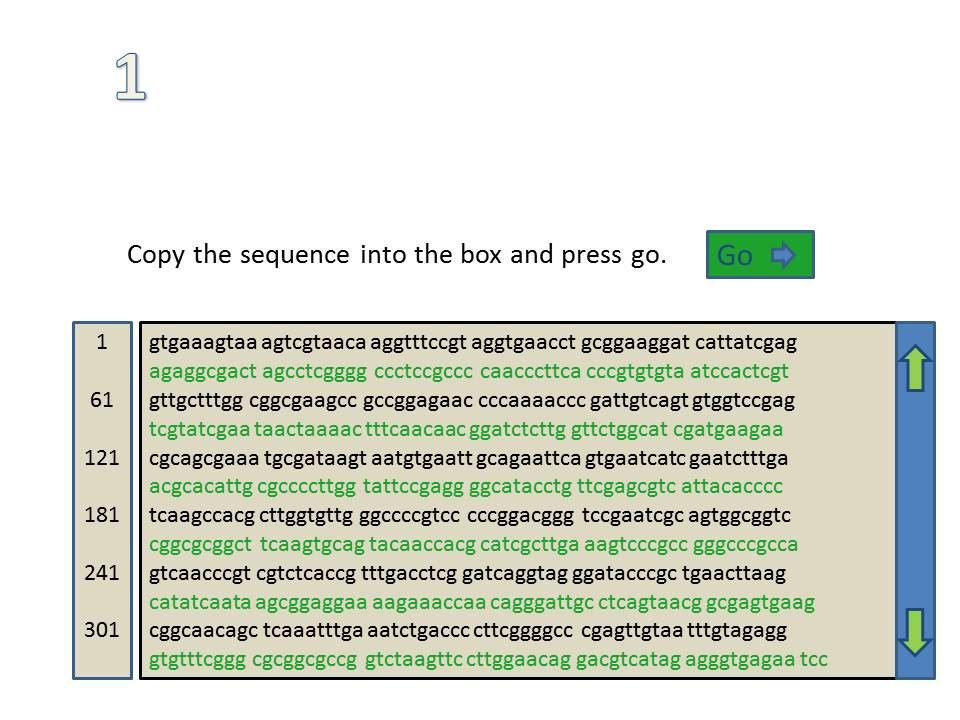
\includegraphics[width=0.6\textwidth]{./images/UiDes/Slide1.jpg}
    \caption{
      \label{fig:UiDes:slide1}
      Initial design, Sequence entry
    }
  \end{center}
\end{figure}

\subsubsection{Specification of target area}
The second slide shows the selection of the DNA sequence part to be amplified by PCR. The user enters the first and the final node numbers in the boxes "From" and "To" respectively, and the chosen area is highlighted after the user presses the "Enter" button. All of the previously introduced functions of the UI, including DNA sequence editing, are present at this stage also. When the user is content with the area specified, he can press the "Go" button to advance to the next stage. The "Go" button color is changed to clearly differentiate from the "Enter" button.

\begin{figure}[h]
  \begin{center}
	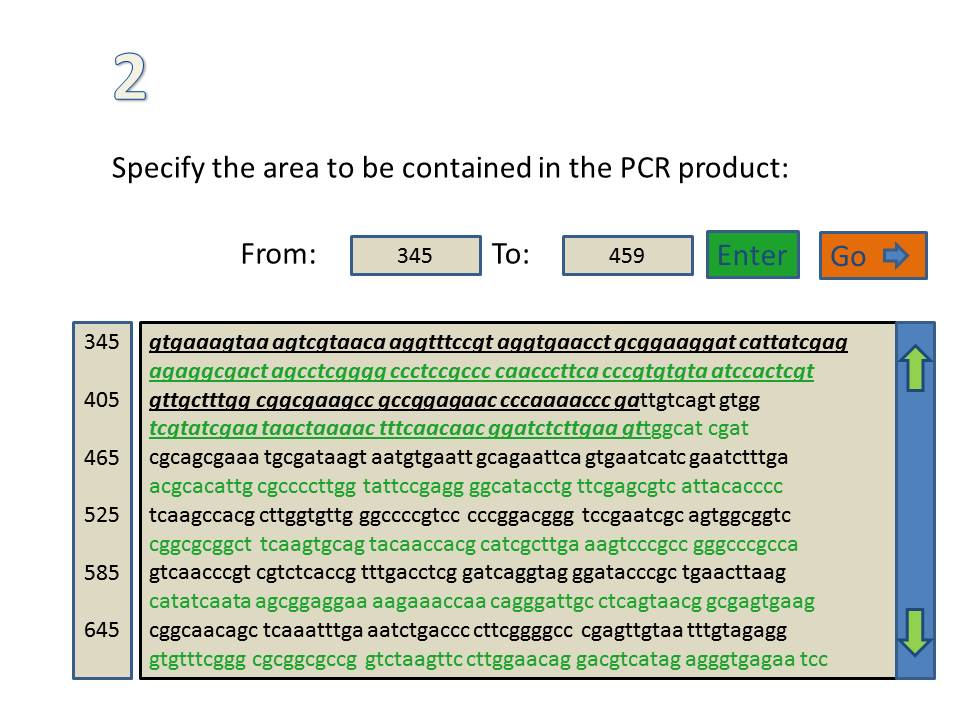
\includegraphics[width=0.6\textwidth]{./images/UiDes/Slide2.jpg}
    \caption{
      \label{fig:UiDes:slide2}
      Initial design,Specification of target area
    }
  \end{center}
\end{figure}

\subsubsection{Primer selection}
Primer selection UI stage is in our view the most important as it is the central part of the exercise, so it is explained extensively by the design document. User is required to copy or type the forward and the backward primers into the boxes above the sequence. The rules of primer design can be viewed by pressing the "Rules" button. If the user decides to change the target area or the sequence itself, he can go back to the previous stage by pressing the "Back" button. 

\begin{figure}[h]
  \begin{center}
	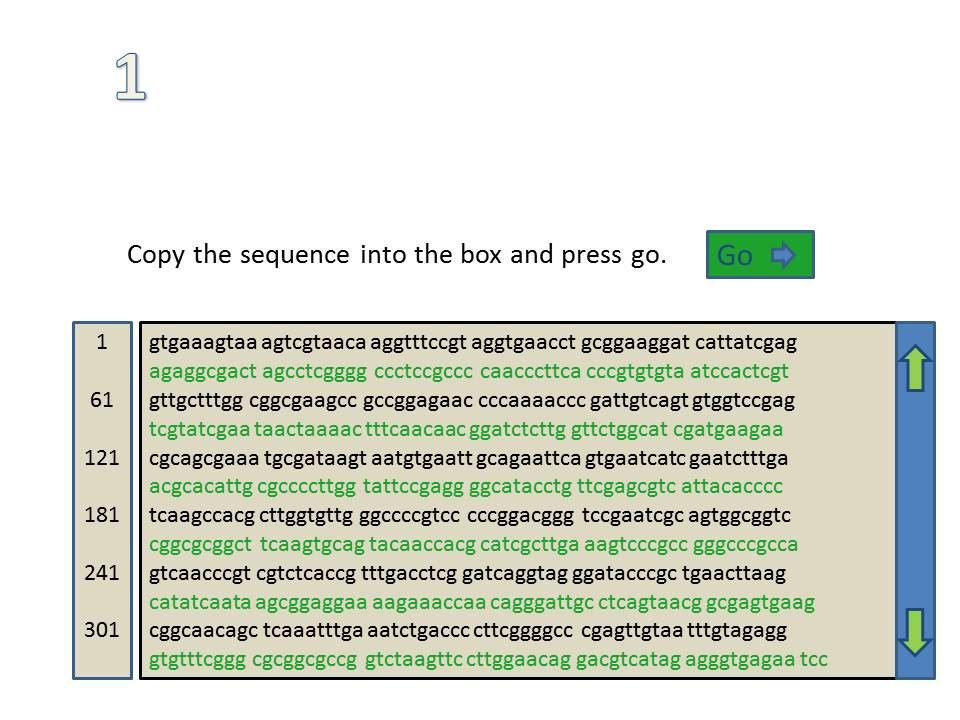
\includegraphics[width=0.6\textwidth]{./images/UiDes/Slide3.jpg}
    \caption{
      \label{fig:UiDes:slide3}
      Initial design, Primer selection - initial screen
    }
  \end{center}
\end{figure}



When the user has entered the primers into their respective boxes, like shown below, he can press the "Go" button to go to the next stage if the primers are correct, or be shown an error message if they aren't.

\begin{figure}[h]
  \begin{center}
	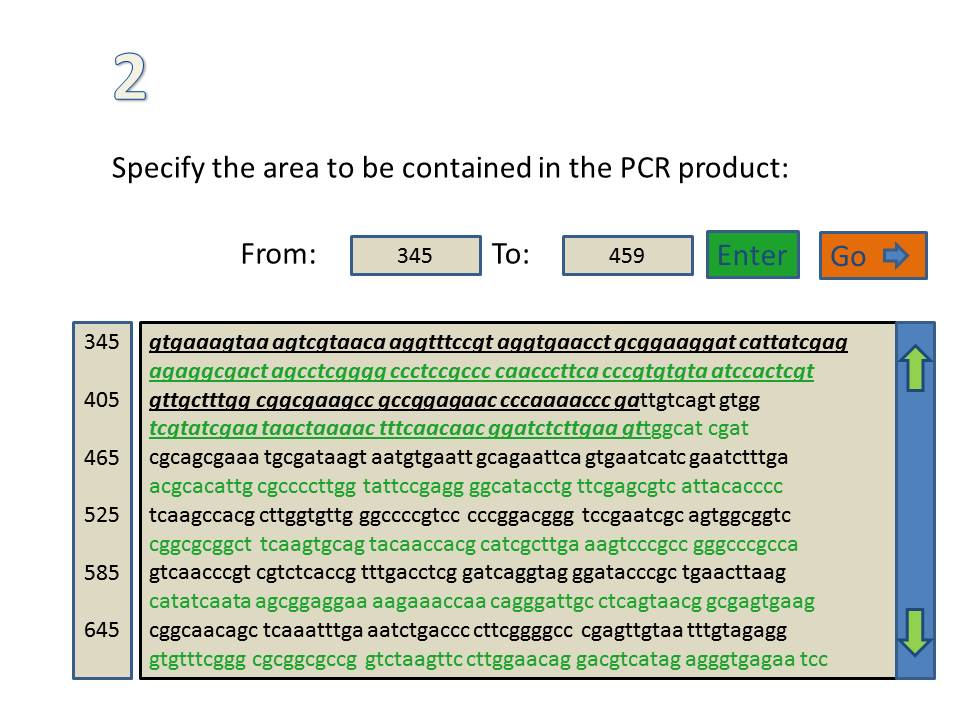
\includegraphics[width=0.6\textwidth]{./images/UiDes/Slide4.jpg}
    \caption{
      \label{fig:UiDes:slide4}
      Initial design, Primer selection - primers entered
    }
  \end{center}
\end{figure}

Each primer is checked for correctness according to the primer design rules and the user is shown a message explaining why his chosen primer is incorrect for the target sequence. In case both primers are incorrect, a separate list of errors is shown for each one. The user can then press the white arrow button to go back to selecting the primers.

\begin{figure}[h]
  \begin{center}
	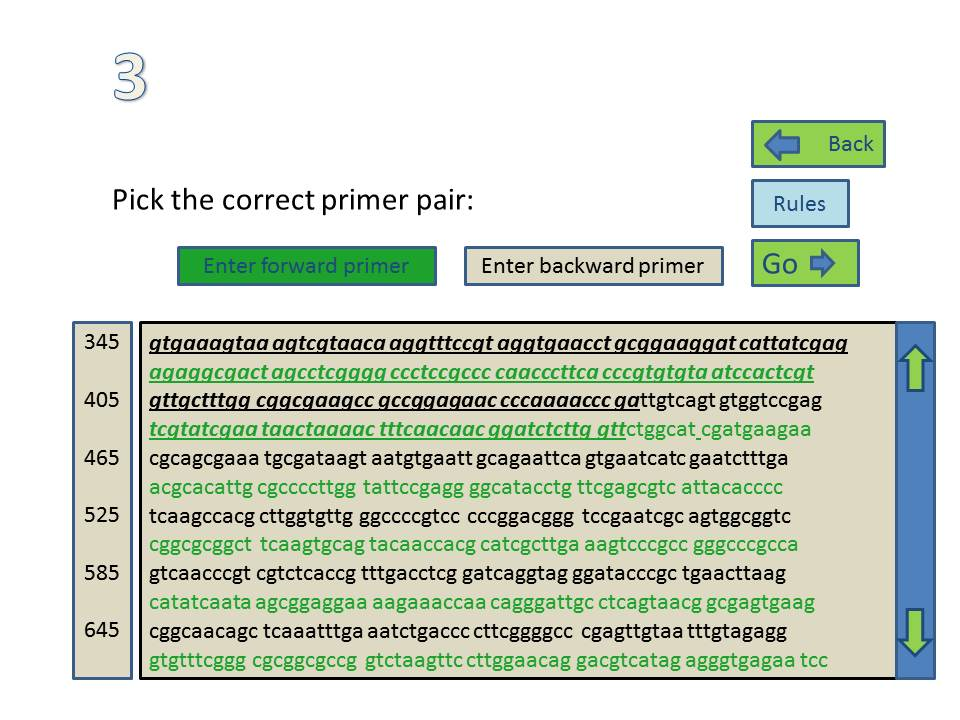
\includegraphics[width=0.6\textwidth]{./images/UiDes/Slide5.jpg}
    \caption{
      \label{fig:UiDes:slide5}
      Initial design, Primer selection - error message
    }
  \end{center}
\end{figure}

\subsubsection{Melting temperature check}
The last slide shows the primers chosen by the user still in their respective boxes and their melting temperatures just below. Both temperatures must be in the range of 50 to 60 degrees Celsium for PCR to work, so if they aren't the user is suggested going back to the previous screen and selecting a different primer pair. As before, pressing "Back" will take the user to a previous stage. The user is also advised to visit the NCBI website (\cite{ncbi}) and performing primer blast on his selected primers to check them for specificity. Lastly, pressing the "Go" button will open a new window with an animation of PCR in action.

\begin{figure}[h]
  \begin{center}
	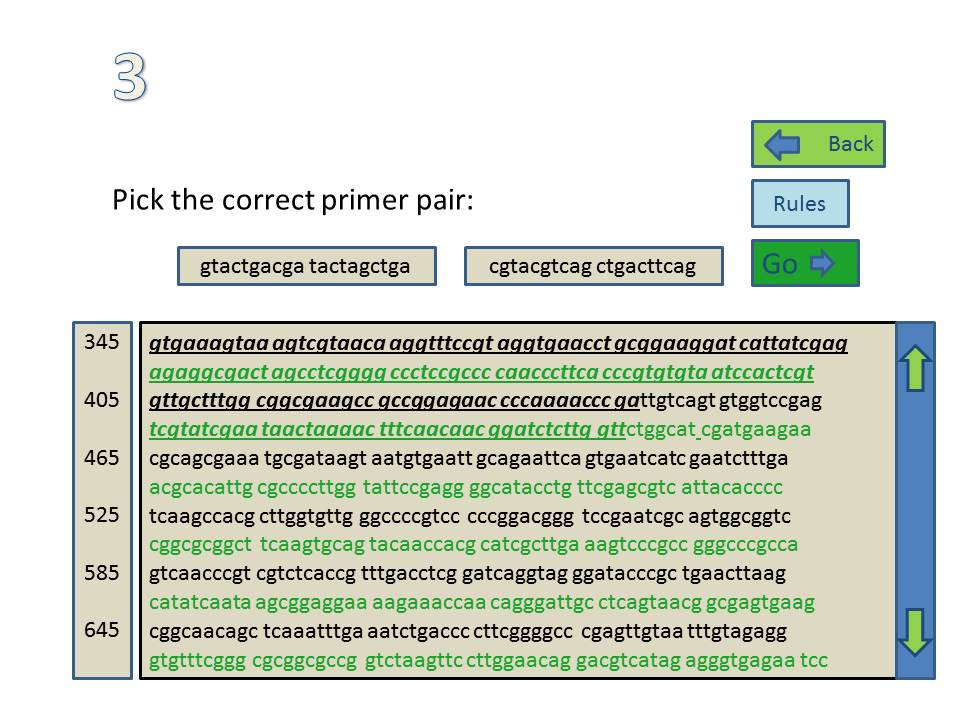
\includegraphics[width=0.6\textwidth]{./images/UiDes/Slide6.jpg}
    \caption{
      \label{fig:UiDes:slide6}
      Initial design, Primer melting temperatures
    }
  \end{center}
\end{figure}



%=====================================================================
\chapter{Implementation}
\label{impl}

\section{Team Distribution}
\label{impl:teamdistribution}
Before the team began implementing the application, we decided to
split the team into three smaller sub-teams, in order to maximise the
use of everyone's time.
These groups were to:
\begin{itemize}
\item Design and implement data models and associated custom methods;
\item Implement the graphical user interface;
\item Design and implement an animation to show the process of PCR.
\end{itemize}

The team's lead programmer, Daniel McElroy, took the lead on this
decision and, while noting each member's particular preferences,
decided to split the team in the following way:
\begin{description}
\item[GUI]{Ross Eric Barnie, Murray Ross}
\item[Data Models and Custom Methods] {Daniel McElroy, Ross Taylor}
\item[Animation] {Dmitrijs Jonins}
\end{description}

While it may have been unnecessary to assign a team-member entirely to
the animation, the team felt that because at the start of the
implementation stage Dmitrijs was out of the country for a prolonged
period of time, that it would serve the team best to give him work he
could complete in his own time.

\section{User Interface}
\label{impl:ui}
The implementation of the graphical user interface (GUI) required a number
of decisions to be made before writing it could begin.

%---------------------------------------------------------------------

\subsection{GUI Framework}
\label{impl:ui:guiframework}

From a brief research period at the start of the implementation 
process, we settled on two possible options for a GUI framework to use
for the application. It is important to note that other GUI options are
available, but based on the team's experience, it became clear that
Swing\cite{swingAPI} or JavaFX\cite{javafxOverview} would be the most
suitable.

%---------------------------------------------------------------------

\paragraph{Swing}
\label{impl:ui:guiframework:swing}

Each member of the group had some limited experience with the Swing 
framework, though not all of it had been positive.
Each member's experience of Swing varied, and
although every member had agreed that their experience had not been
entirely problem-free, we conceded that its integration with the NetBeans
Integrated Development Environment (IDE), discussed in section
\ref{impl:ui:ide:netbeans}, was extremely useful.

However, on investigating the framework more closely it was clear that
Swing was extremely well documented with full API specification
\cite{swingAPI}, and in-depth tutorials \cite{swingTutorial}.
This was a key element of our decision as we felt that the documentation
provided would be more than adequate to enable us to use the framework
with relative ease.

%---------------------------------------------------------------------

\paragraph{JavaFX}
\label{impl:ui:guiframework:javafx}

Another framework considered was JavaFX, with which no member of the team
had any experience. 
Some members felt that this was a risk worth taking, given the challenges
faced in previous experiences with Swing.
In reality, JavaFX was only briefly considered and totally disregarded
when, upon investigation, we discovered that JavaFX was still a relatively
new framework, and consequently, comprehensive documentation was not as
readily available for JavaFX as with Swing, particularly when it came 
to troubleshooting on online forums.

In addition, JavaFX required Java 7, which, again, no member of the
group had used before and which at the time was not available in the
Level 3 Laboratory where we would be working for the majority of the
year.
It seemed like too much of a risk to try to learn two different
technologies at the same time, while having to provide our own
development platforms, which, with various members of the team never
having used the Linux OS before, could potentially cause a number of
problems.

%---------------------------------------------------------------------

\subsubsection{Decision}
\label{impl:ui:guiframework:decision}

The investigation was carried out by the group's Toolsmith, Ross
Barnie, who presented the evidence discussed in the sections above
regarding the two frameworks to the rest of the team.
With this evidence the team voted in favor of using the Swing
framework with Java 6.

Retrospectively, Swing and Java 6 are out-of-date technologies and
JavaFX is now packaged with Java 7 \cite{javafxOverview}, so the
application would have been more up-to-date or future-proof had we
used JavaFX.
Additionally, many of the computers in the level 3 lab now do have
Java 7 installed upon another project team requesting it, so our fears
over development platform problems were nullified, though this was
only after we had started development and could not have been foreseen.

It was an unfortunate shortcoming of the research into JavaFX that the
group did not know about JavaFX's integration with the NetBeans IDE
which was seen as one of the key differences between the two
frameworks at the time of making the decision.

%---------------------------------------------------------------------
%---------------------------------------------------------------------

\subsection{Integrated Development Environment (IDE)}
\label{impl:ui:ide}

One concern was that, in some members' experience, using two separate
IDEs was extremely time consuming, particularly while using version
control.
This was mostly due to various metadata that IDEs keep track of in
various files, however this meant that any small change to the source
code would change the metadata and therefore each commit would have to
involve adding it, which would be very time-consuming.

It is because of this experience that the group decided to work from a
single IDE, researched again by Ross Barnie.

%---------------------------------------------------------------------
\paragraph{NetBeans \cite{netbeans}}
\label{impl:ui:ide:netbeans}

NetBeans is an IDE which the team had had little experience with and had
only used in the context of building applications with GUIs created
using the Swing framework.
There was some trepidation to using NetBeans since most of the team
had associated their problems with Swing with NetBeans itself.
Upon further research, which involved using the IDE to build small
applications, NetBeans started much faster than Eclipse, discussed
below.
The design interface was also very simple and easy to use, with each
element being laid out the way you wish and the associated source code
being generated for you.
This meant that the design layout could be finished very quickly,
rather than spending our time writing hundreds of lines of source code
just for the interface.

NetBeans' metadata was minimal so would not clutter the version
control repository to an unacceptable degree.

%---------------------------------------------------------------------
\subsubsection{Eclipse \cite{eclipse}}
\label{impl:ui:ide:eclipse}

The team had substantial knowledge of Eclipse from its mandated use in
Java Programming 2 \cite{javaProgramming2}. Again, our experience of 
Eclipse is somewhat tainted by associations with problems we faced at 
the time, such as a bug on the version for Windows which meant that 
Eclipse would freeze if you tried to copy or paste anything.

In our experience, we found Eclipse to be very slow, both during 
start-up and normal operation. 
Editing-wise, Eclipse was rather cumbersome and had few benefits over
a text editor.
Also, the requirement to bind the ``Workspace'' was seen as a potential
point for confusion and errors.

In addition, the team felt that the missing design interface seen on
NetBeans, discussed above, was a huge disadvantage and would cause a
significant loss of time, simply due to the volume of code we would
have to write instead of being auto-generated.

Members of the team also pointed out that Eclipse has a tendency to
create a large amount of metadata which would clutter the version
control repository.

%---------------------------------------------------------------------
\subsubsection{No IDE}
\label{impl:ui:ide:noide}

It was briefly considered to have no IDE at all and simply use text
editors.
This would allow for extremely fast editing in a very comfortable
environment, since most text editors, such as Vim \cite{vim} or Emacs
\cite{emacs}, are highly customisable and can launch in a matter of
seconds.
Text editors would also not require metadata, keeping our version
controlled directories clean.

However, the obvious problem with no IDE is that troubleshooting
source code problems without any real-time error-checking like in IDEs
is more difficult and, unlike with IDEs, you cannot automatically
import a missing package or method, nor can there be any
auto-generated code at all for that matter.

%---------------------------------------------------------------------
\subsubsection{Decision}
\label{impl:ui:ide:decision}

When the evidence above was given to the team, we were also discussing
which GUI Framework to use (as discussed in section
\ref{impl:ui:guiframework}) and it became obvious that integration
with the framework would be key to helping us develop the GUI.

We therefore decided to work with the NetBeans IDE because of the
design interface, minimal metadata, and lack of (known) bugs that
would affect us in any meaningful way.

Retrospectively, this was the correct decision.
Even if we had chosen a different GUI framework, the advantages of the
easy-to-edit design interface far outweigh any problems we had with
it.

%---------------------------------------------------------------------
\subsection{Builds}
\label{impl:ui:builds}

To demonstrate the GUI and the changes we made to it over time, we
will discuss two builds of the system at two crucial points in time.

The first is what the team refer to as the ``demo build'', which was
the first build of the system in general to be used by anyone outwith
the project.
It was, at the time, the most up-to-date version of the program and is
called the demo build since it was used in a demonstration (discussed
in section \ref{eval:demo}) on 8th February 2012.

The second is the current build of the system, which is currently
linked to on the Molecular Methods moodle site to be used by any of
its 160 students.
This build by nature has developed from the demo build in that most of
the changes made were based on the evaluation and feedback we received
from the demonstration itself (discussed in section \ref{eval:demo}).
%---------------------------------------------------------------------
%---------------------------------------------------------------------

\subsubsection{Demo Build}

%---------------------------------------------------------------------
\paragraph{Overview}

Before the demonstration, the team were asked to include an
``overview'' panel to tell the user what they can expect from the
application, as well as show the primer design rules to remind the
user about them.
This can be seen in figure \ref{fig:demoBuild:splash}.

Its design is to maximise the separation of concerns, so the Overview
section is to the left, which due to the way English is read, is the
more likely of the three sections to be read first, at least by fluent
English readers.
In this overview section it was decided to include contact details
of the team in case the user found technical problems with the
program since, as discussed in section \ref{eval:future}, the
team plan on maintaining the system for future use.

\begin{figure}[!t]
  \begin{center}
    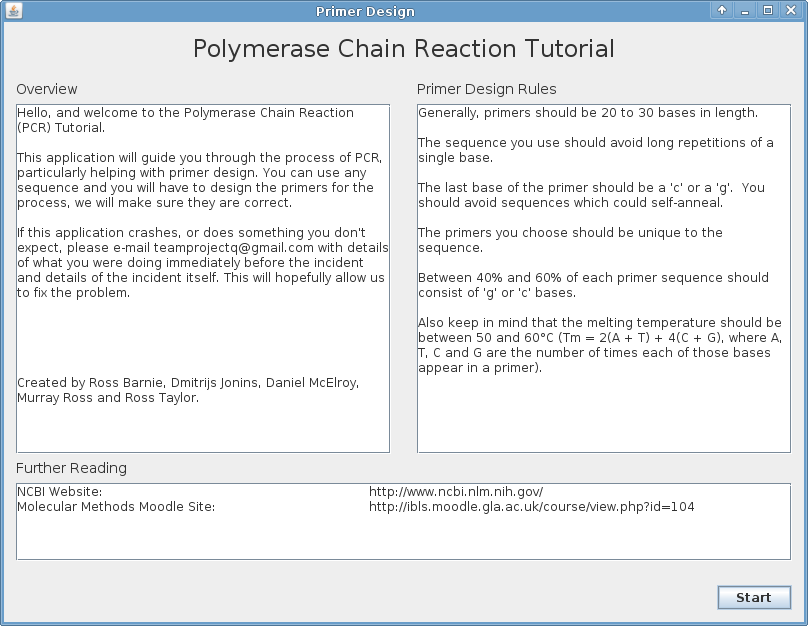
\includegraphics[width=0.6\textwidth]{./images/demoBuild/splash.png}
    \caption{
      \label{fig:demoBuild:splash}
      Demo Build, Overview Panel 
    }
  \end{center}
\end{figure}

\paragraph{Sequence Entry}

\begin{figure}[!t]
  \begin{center}
    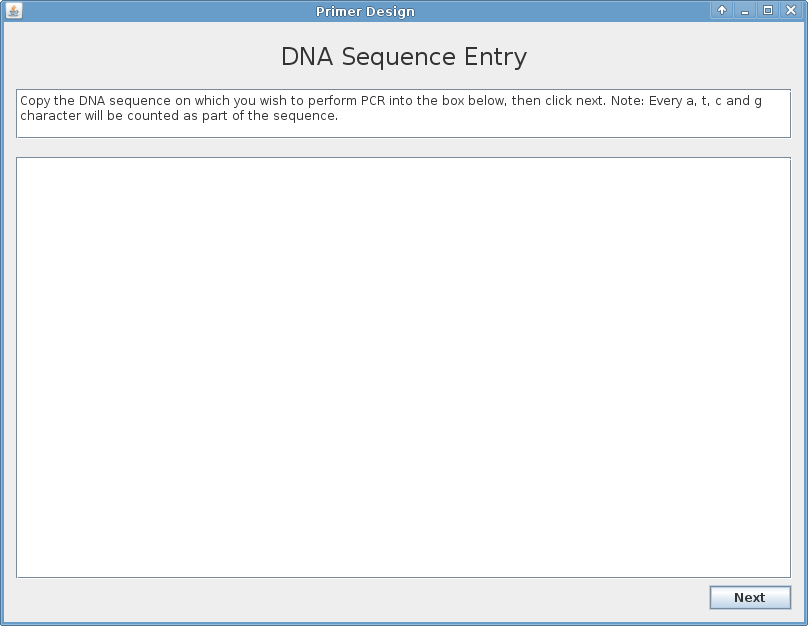
\includegraphics[width=0.6\textwidth]{./images/demoBuild/sequenceEntry.png}
    \caption{
      \label{fig:demoBuild:sequenceEntry}
      Demo Build, sequence entry panel 
    }
  \end{center}
\end{figure}

Figure \ref{fig:demoBuild:sequenceEntry} shows the next panel,
referred to by the team as the ``sequence entry'' panel.
While based on the design discussed in Section \ref{design:ui} it
has been altered slightly to maximise the amount of space to be used
for entering in the sequence, as this is the primary purpose of this
panel.

It was expected of the user to go to the National Center for
Biotechnology Information \cite{ncbi} website and obtain a DNA sequence by
copying it to their clipboard and then pasting this into the sequence
entry panel and this was explained in the accompanying user guide (see
documentation).
Although this relied heavily on the users' ability to use keyboard
shortcuts, it was assumed that all students at university level would
at least have an awareness of these shortcuts.
We also assumed that once students were told of these shortcuts, as
they were in the user guide, that they would be comfortable using
them.

%---------------------------------------------------------------------

\paragraph{Target Selection}

\begin{figure}[!t]
  \begin{center}
    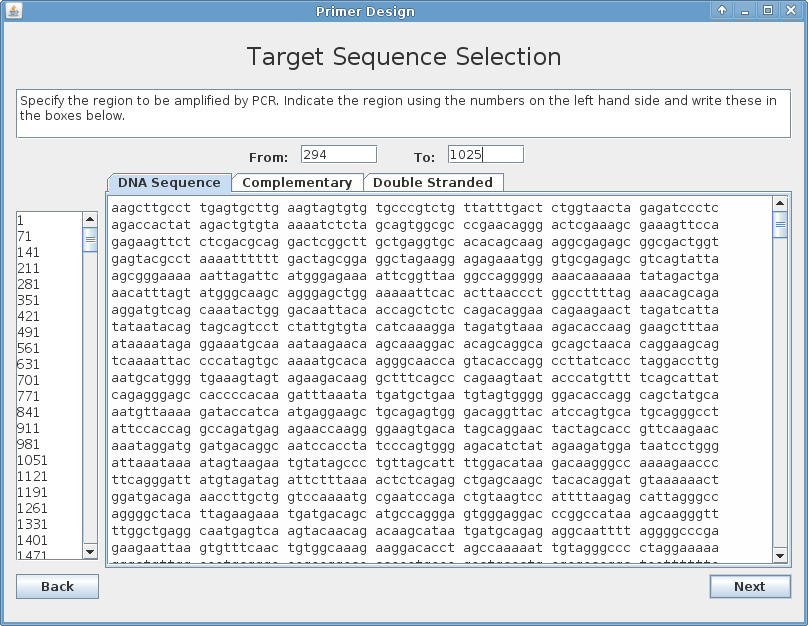
\includegraphics[width=0.6\textwidth]{./images/demoBuild/areaSelection.png}
    \caption{
      \label{fig:demoBuild:areaSelection}
      Demo Build, Target Selection Panel
    }
  \end{center}
\end{figure}

Following the Sequence Entry panel is the ``Target Selection'' panel,
shown in figure \ref{fig:demoBuild:areaSelection}, which requires the
user to specify the sequence that they wish to amplify, or the
``target'' sequence.
%This is accomplished by the user entering the start and end of the 
%required area of the sequence index of these bases, into the ``From'' 
%and ``To'' fields at the bottom of the panel.
In order to select the target sequence, the user must enter the index
of the first base of the target into the ``From'' text field, and the
index of the last base of the target into the ``To'' text field.


Finding the indices would, ideally, be aided by the text pane at the 
left of the screen which shows the base number of the first base on its 
line. Unfortunately, for unknown reasons, the text panes became 
misaligned when viewed from any platform other than the current 
development platform (the level 3 Computing Science Laboratory computers
running Scientific Linux \cite{scientificLinux}) and this misalignment
can be seen in figure \ref{fig:demoBuild:areaSelection}.

An addition made to the original design discussed in Section
\ref{design:ui} is the tabs above the main text area, which allow the
user to switch between the sequence they entered, and its
complementary equivalent, generated by the program.
It was suggested by the clients to have this feature as it would
greatly increase the speed at which the user could design the reverse
primer since this is based on the complementary strand.
Without the complementary tab, not only would the user have to
manually convert the primer to its complementary equivalent, but also
reverse its order, which neither the team nor the clients felt was a
useful way for students to spend their time. 

%---------------------------------------------------------------------

\paragraph{Primer Design}

Following the Area Selection panel is the ``Primer Design'' panel,
shown in figure \ref{fig:demoBuild:primerDesign}, which allows the
user to enter forward and reverse primers.

\begin{figure}[!t]
  \begin{center}
    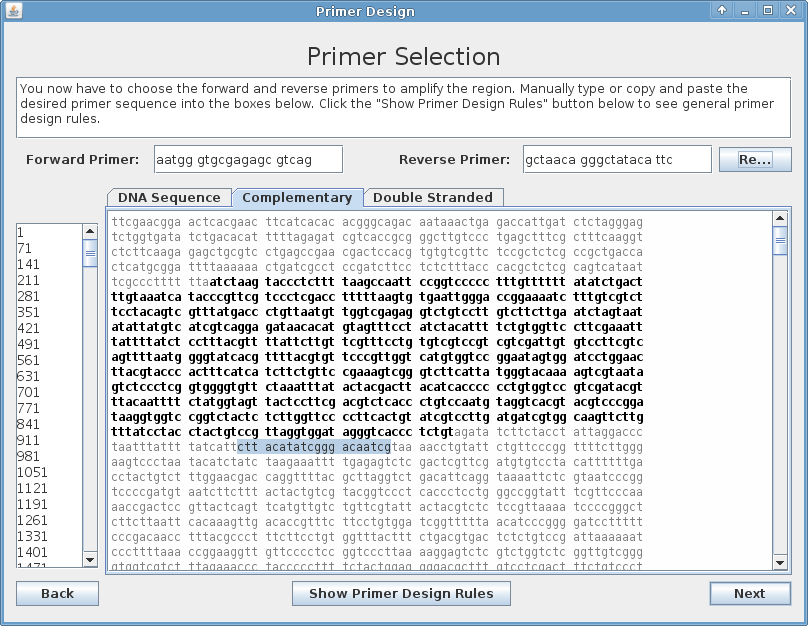
\includegraphics[width=0.6\textwidth]{./images/demoBuild/primerDesign.png}
    \caption{
      \label{fig:demoBuild:primerDesign}
      Demo Build, Primer Design Panel
    }
  \end{center}
\end{figure}

One of the design features we had intended to provide was ``dynamic
highlighting'', as it was referred to by the team.
This would highlight the user-entered primers (from the ``Forward
Primer'' and ``Reverse Primer'' text fields) within the sequence in
the center of the panel, showing the user where their primer lies
within the sequence.
This highlighting was unfortunately missing in the demo build due to
time constraints.

However, we had always intended to give feedback to the user should
they break rules of primer design and the demo build version of this
can be seen in figure \ref{fig:demoBuild:primerFeedback} and appears
when the user clicks the ``Next'' button.
Again based on the design (section \ref{design:ui}), this dialogue
window shows the user any rules which they have broken, and which
primer the feedback is referring to.

\begin{figure}[!t]
  \begin{center}
    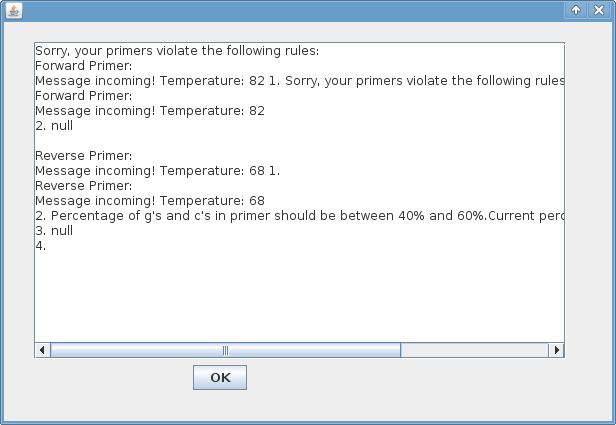
\includegraphics[width=0.6\textwidth]{./images/demoBuild/primerFeedback.png}
    \caption{
      \label{fig:demoBuild:primerFeedback}
      Demo Build, Feedback on User-entered Primer
    }
  \end{center}
\end{figure}

Again, due to time constraints this was not as fully featured as we
had hoped for in the demonstration, however it did display enough
information to give an idea to our clients of what the feedback might
look like in the future (see further discussion in section
\ref{eval:demo}).

In order to design a reverse primer outwith the system, the
complementary strand would have to be calculated (which would be in
the 3'---5' direction) and reversed to be in the correct direction
(5'---3').
In the application, the complementary strand is already calculated, so
the user can simply copy and paste a primer of their choosing from the
sequence and put it in the reverse primer text field.
However, this does not solve the problem of reversing it, so the
``Reverse'' button was put next to the reverse primer text field,
which intuitively reverses the order of the primer in the text
field. 

At the bottom of the panel in the middle of the ``Back'' and ``Next''
buttons is the ``Primer Design Rules'' button, which shows,
intuitively enough, the primer design rules set out at the beginning
of the program.
This was part of the initial design, the button for which can be seen
in figure \ref{fig:UiDes:slide3} and the implementation of which can
be seen in figure \ref{fig:demoBuild:primerDesignRules}.

\begin{figure}[!t]
  \begin{center}
    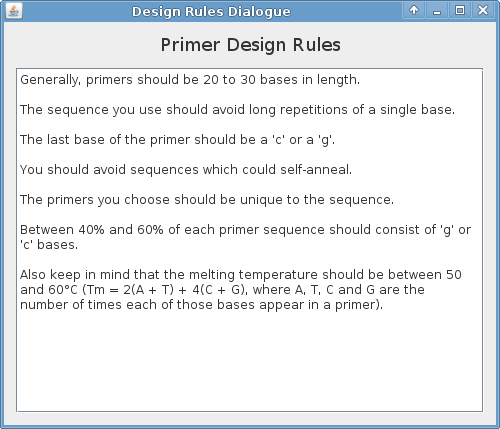
\includegraphics[width=0.6\textwidth]{./images/demoBuild/primerDesignRules.png}
    \caption{
      \label{fig:demoBuild:primerDesignRules}
      Demo Build, Primer Design Rules Dialogue
    }
  \end{center}
\end{figure}

\paragraph{Melting Temperature}

After designing a primer, the user is presented with the ``Melting
Temperature'' panel as seen in figure \ref{fig:demoBuild:meltingTemp}
for the user to evaluate their primers.

In the case of the demonstration, this panel was blocked from the user
unless they had a correct primer.

\begin{figure}[!t]
  \begin{center}
    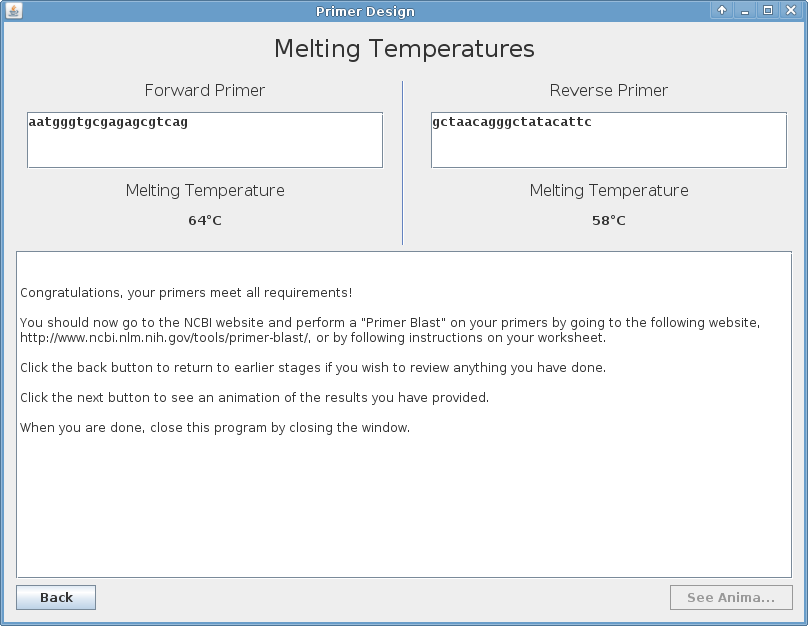
\includegraphics[width=0.6\textwidth]{./images/demoBuild/meltingTemp.png}
    \caption{
      \label{fig:demoBuild:meltingTemp}
      Demo Build, Melting Temperatures of User's Primers.
    }
  \end{center}
\end{figure}

While the initial design \ref{design:ui} was sufficient as a mock-up,
it lacked consistency with the rest of the program.
It also proved difficult to reproduce in Swing with the NetBeans
Design view while maintaining the professional appearance of the rest
of the program.
Initial attempts had JLabel objects, all misaligned, spread very
sparsely around the panel and looked very rushed and unprofessional.

The demo build version addresses the problems we faced in these initial
attempts by using a single large text box to display all the necessary
information to the user about possible future work and the upper
section of the panel to provide the user with the ability to review
their primers. 
Thus reducing the amount of unused space on the panel,
while also keeping it consistent (with the traversal buttons on the
bottom of the panel) with the rest of the program.

The emphasis on the primers and the melting temperatures in bold means
that the user can easily see their primers and the associated melting
temperatures, while the separator down the center visually separates
the forward from the reverse primer.

Unfortunately the animation was not available in time for the
demonstration and although the button for it was included in this
panel, it was disabled.

%---------------------------------------------------------------------

\subsubsection{Current Build}

Addressing feedback from the demonstration (see section \ref{eval:demo}),
and adding new elements to provide extra functionality, the current
build is several iterations ahead of the demo build discussed above
and is currently available to all Molecular Methods students.

While there have been many changes to the build in this time, there
have been few alterations to the UI as most feedback about it at the
demonstration was positive.
Most changes stem from evolving requirements or from the
demonstration feedback.

\paragraph{Overview}
The overview panel (seen in figure \ref{fig:demoBuild:splash})
changed only because of the addition of the menu bar, discussed
below.
It was felt that this needed very little change, if any, from the demo
build and is therefore identical to the demo build version in almost
every respect.

\paragraph{Sequence Entry}

\begin{figure}[!t]
  \begin{center}
    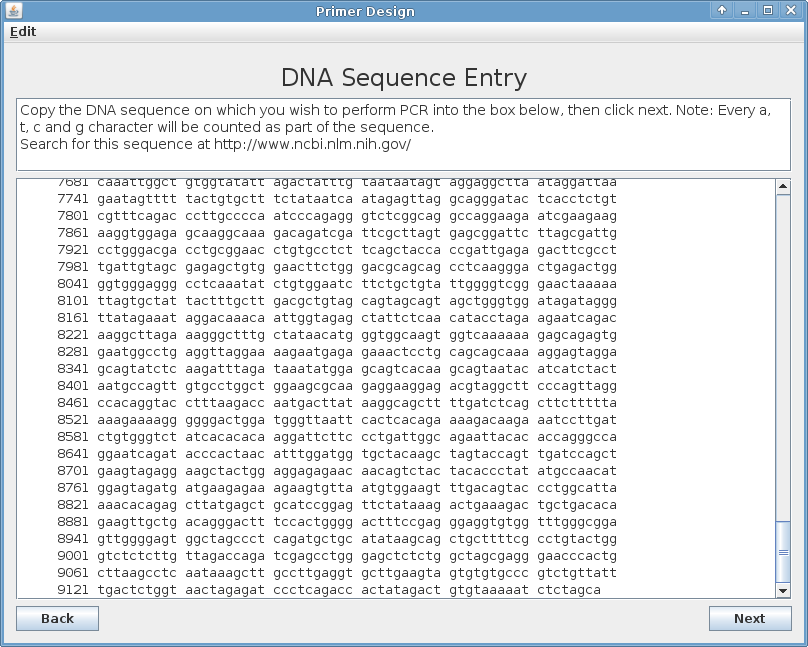
\includegraphics[width=0.6\textwidth]{./images/currentBuild/sequenceEntry.png}
    \caption{
      \label{fig:currentBuild:sequenceEntry}
      Current Build, Sequence Entry Panel
    }
  \end{center}
\end{figure}

In terms of changes made after the demo build, this panel is similar
to the Overview panel above in that neither have been changed to any
significant degree.

However, as can be seen in figure \ref{fig:currentBuild:sequenceEntry}
there have been some minor changes.

\begin{itemize}
\item The menu bar at the top of the panel, which was added to
address the issue of people not being familiar with keyboard
shortcuts.
The menu itself was named ``Edit'' to conform to standards set by most
applications with menu bars in that the ``Copy'' and ``Paste''
features are usually found under the ``Edit'' menu.

\item The ``Back'' button on this panel which was not present for
the demo build.
For the demo build, the inclusion of a back button felt unnecessary as
any information that users would require in order to use the 
program is available throughout the application (for example, Primer Design 
Rules is available on Primer Design panel, and the NCBI website \cite{ncbi}
is given to user in the instructions underneath the panel title).
However, the clients felt the ``Back'' button was a necessary inclusion, and
we were more than happy to defer to their insight.
\end{itemize}

\paragraph{Target Selection}

\begin{figure}[!t]
  \begin{center}
    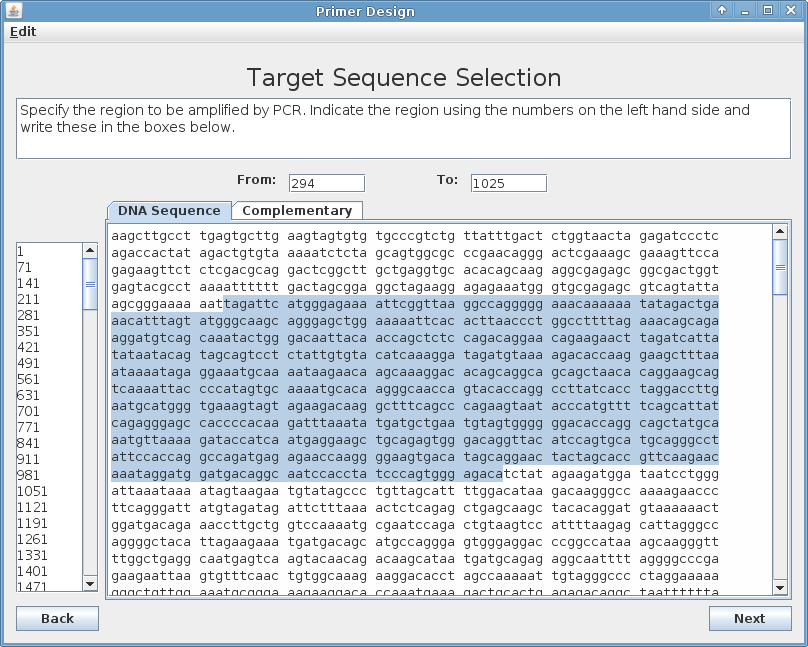
\includegraphics[width=0.6\textwidth]{./images/currentBuild/areaSelection.png}
    \caption{
      \label{fig:currentBuild:areaSelection}
      Current Build, Target Selection Panel
    }
  \end{center}
\end{figure}

While the interface of the Target Selection panel may not have changed
drastically from the demo build, the way a user selects the target has
changed to make the process much easier.

Previously, as discussed in section \ref{fig:demoBuild:areaSelection},
the user would have to find the indices of the start and end bases of
the target.
Now, as can be seen in figure \ref{fig:currentBuild:areaSelection},
the user simply has to highlight the desired sequence and the indices
are calculated automatically.
This change means that users do not have to depend on the
aforementioned unreliable line numbers (see Section
\ref{eval:future}), and can focus instead on the actual sequence.
It also provides a clearer visual reference to the user's sequence,
without the need to switch between this and the next panel, which was
one of the issues brought up in the demonstration (see Section
\ref{eval:demo}).

\paragraph{Primer Design}

\begin{figure}[!t]
  \begin{center}
    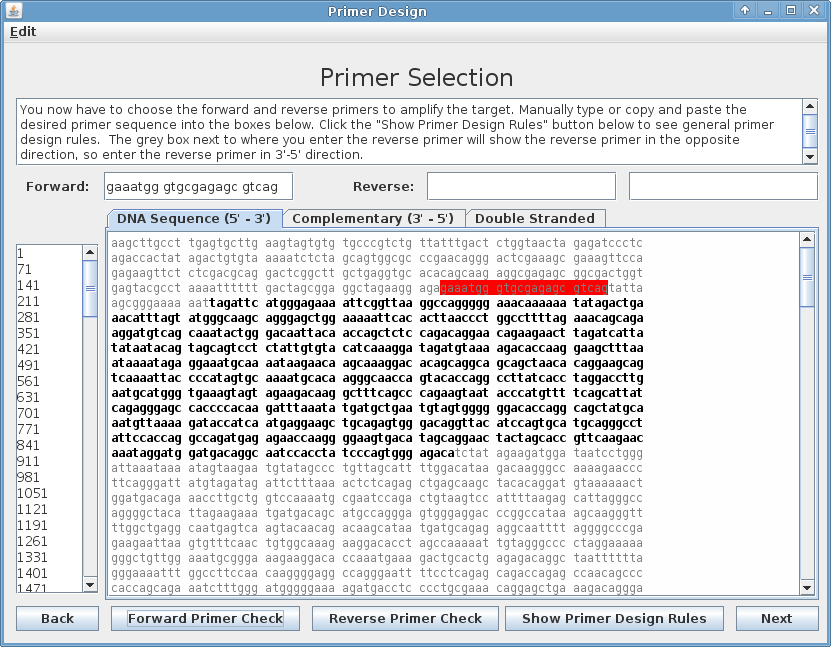
\includegraphics[width=0.6\textwidth]{./images/currentBuild/forwardPrimerDesignRed.png}
    \caption{
      \label{fig:currentBuild:forwardPrimerDesignRed}
      Current Build, (Forward) Primer Design, showing invalid primer selection
    }
  \end{center}
\end{figure}

Primer design received a lot of attention in that it received the
majority of new features in the application since the demo build.

Firstly, a feature referred to by the team as ``dynamic highlighting''
which, when a user enters a sequence of characters in to the primer
text fields, highlights that sequence within the larger sequence.
This can be seen in figure
\ref{fig:currentBuild:forwardPrimerDesignRed}.
Initially, this highlighting was going to consist of a single colour, 
simply to help the user see if the primer is unique to the sequence, 
and so that they can visualise where the primer is within the sequence.
The lack of visual aids in the demo build was something we strove to
rectify especially after the feedback from the demonstration (section
\ref{eval:demo}).
To this end, we also made the highlighted sequence change colour depending 
on the correctness of the primer. How this is decided is discussed in 
section \ref{impl:models:dynHigh}.
This can be seen in figure \ref{fig:currentBuild:forwardPrimerDesignRed} 
with an incorrect primer, and figure \ref{fig:currentBuild:forwardPerfectPrimer} 
with a perfect primer.

\begin{figure}[!t]
  \begin{center}
    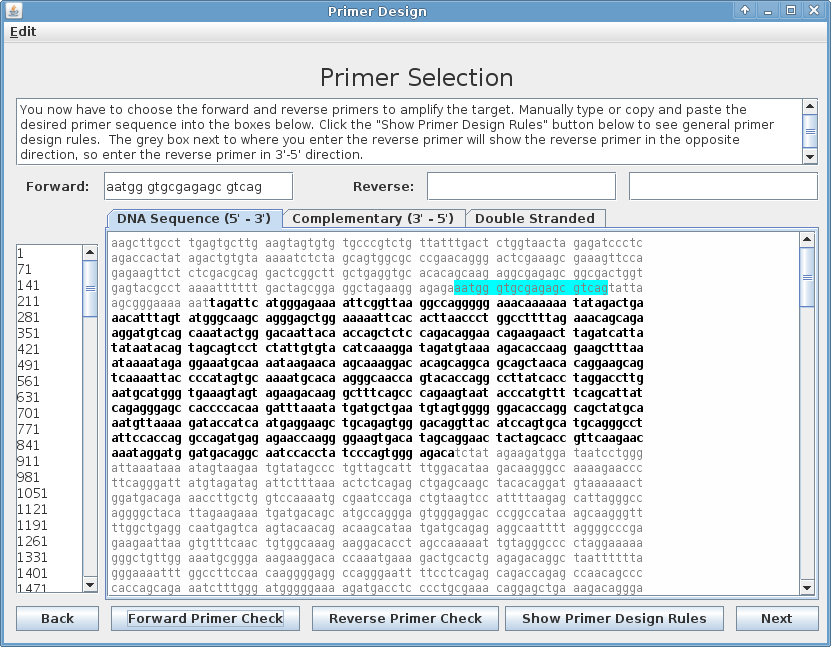
\includegraphics[width=0.6\textwidth]{./images/currentBuild/forwardPerfectPrimer.png}
    \caption{
      \label{fig:currentBuild:forwardPerfectPrimer}
      Current Build, (Forward) Primer Design, showing perfect primer selection
    }
  \end{center}
\end{figure}

Another new feature added based on the demonstration feedback was the
two new buttons at the bottom of the panel, which give feedback on a
single primer, depending on which button the user presses.
An example of what that feedback looks like can be seen in figure
\ref{fig:currentBuild:primerEvalRed}.

\begin{figure}[!t]
  \begin{center}
    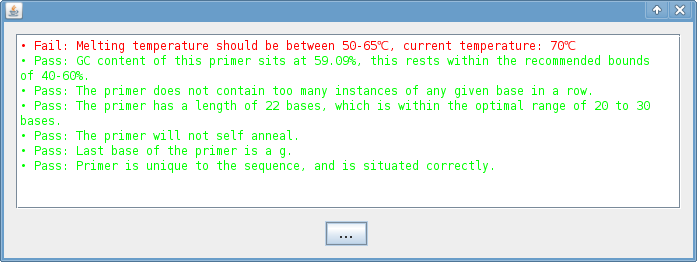
\includegraphics[width=0.6\textwidth]{./images/currentBuild/primerEvalRed.png}
    \caption{
      \label{fig:currentBuild:primerEvalRed}
      Current Build, Single Primer Feedback
    }
  \end{center}
\end{figure}

This feedback is also colour-coded to make any problems with the
user's primer(s) more immediately apparent than in the demo build.

With the emphasis on direction of the sequence being made more obvious
in this version with the direction shown in the tab names, it is more
obvious as to which direction the user should be thinking about when
creating the reverse primer.
To allow the user to only have to think about one direction, the
``Reverse'' button from the demo build was replaced by an uneditable
text field which auto-generates the reverse order of the reverse
primer, see figure \ref{fig:currentBuild:reversePrimerPerfect}.
It was also ambiguous, when the reverse button was in place, whether
the primer in the text field had been reversed or not. 
For example, if the user were to press the reverse button more than
once, the user would have to remember this and there was nothing in
the interface to remind them, relying heavily on the user's recall.

\begin{figure}[!t]
  \begin{center}
    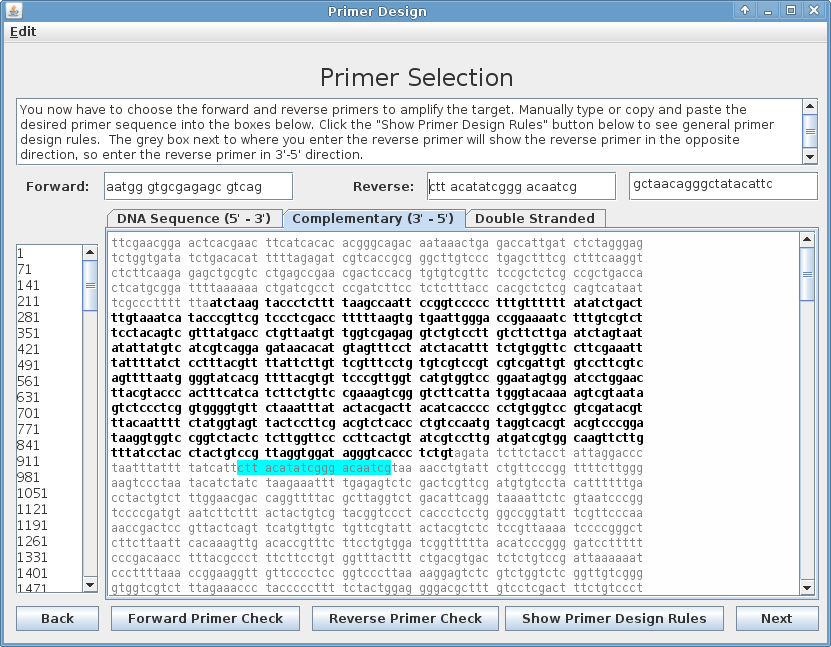
\includegraphics[width=0.6\textwidth]{./images/currentBuild/reversePrimerPerfect.png}
    \caption{
      \label{fig:currentBuild:reversePrimerPerfect}
      Current Build, Reverse Primer (showing perfect primer)
    }
  \end{center}
\end{figure}

When the user clicks the ``Next'' button, they are presented with a
dialogue window, giving the user a list of comments on each rule of
primer design, with a rating of ``pass'', ``fail'' or ``close fail''
for how their primers performed against these rules, an example of
which can be seen in figure
\ref{fig:currentBuild:primerDesignBothFeedback}.
Again, these are colour-coded to make broken rules stand out to the
user.

The feedback given at this stage confirms to the user that their
primers conform to all primer design rules to an acceptable degree and
lets the user know that their primers were correct.

\begin{figure}[!t]
  \begin{center}
    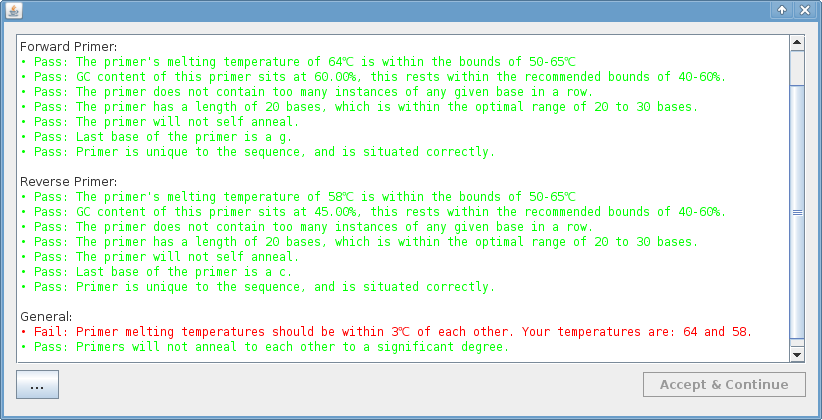
\includegraphics[width=0.6\textwidth]{./images/currentBuild/primerDesignBothFeedback.png}
    \caption{
      \label{fig:currentBuild:primerDesignBothFeedback}
      Current Build, Feedback on both primers dialogue
    }
  \end{center}
\end{figure}

%---------------------------------------------------------------------
\subsubsection{Comparison}

Overall the two builds appear very similar in that they are laid out
in a very similar way and the designs were not radically changed.
However all of the minor changes and additional functionality made a
huge difference overall.

\paragraph{General}
Each panel, or more accurately the shared JFrame object (the window
shared by each panel), now has a menu bar with the Edit menu so that
users do not have to rely on the keyboard shortcuts for copy and
paste, which was an additional requirement set out by the clients and
from the demonstration feedback.
Many people do not frequently use keyboard shortcuts so this gives
users a graphical way of copying and pasting data to and from the
application.

\paragraph{Overview}
The overview was given positive praise in the demo build, the only
change being a larger ``Start'' button since this was noted by the
clients as being too small for users to immediately notice.

\paragraph{Sequence Entry}
Again, this panel has received little attention since the demo build
since it served its purpose well.
The only change was to the instructions text pane just under the title
since the instructions were too minimal during the demo and a back
button was added to ensure the user could traverse the program in its
entirety and see the ``Further Reading'' text pane for useful links at
any point during the program.

\paragraph{Target Selection}
With the addition of the automatic index entry via text highlighting
functionality users, and teaching staff, now have more options for
entering a target.
For example, a user can quickly and easily select a sequence that they
wish to amplify by highlighting it in the text, rather than having to
count the indices as they had to in the demo build which was a slow
and tedious process.
While teaching staff could produce an accompanying tutorial or
assessment specifying that the user must use a particular sequence
with a specific, allowing greater versatility in the manner in which
the program is used as this could be used as a lab exercise.

\paragraph{Primer Design}
Selecting a primer in the demo build was a guessing game in that the
user could never deduce for themselves whether a primer they entered
was unique, for example, since no visual cues were given.
Primer rules would be broken and the user would be told this but with
only the rules, which at the time were only allowed to pass or fail,
and no colour-coding, the design in general failed to stimulate and
teach.
Another issue was the ambiguity of whether the reverse primer had been
reversed or not by the reverse button.

With the primers now being highlighted within the sequence it is easy
to tell if the primer is unique, the colour-coding allows the user to
instantly see how their primer is evaluated against the primer design
rules without the need to check it using the primer check buttons
every time and the reverse button has been replaced to reduce
ambiguity and emphasise the sequence direction, adding to users'
understanding. 

Primers can also now be checked individually so that the user can
check one primer as they enter it, rather than having to read the same
feedback repetitively while working on a completely separate primer.

\paragraph{Melting Temperatures}
Cosmetically, the melting temperature panel did not need any changes
since it served its purpose of letting the user evaluate their primers
well.

Of course, the difference between the demo build and the current build
in terms of this panel is that the animation is now available and thus
the ``See Animation'' button has been enabled.



\section{Models \& Custom Methods}
\label{impl:models}

\subsection{Models}
%- 3 objects, Sequence, Primer, TestResult
%Basic in construction, all classes have toStrings and booleans.

\begin{figure}[!t]
  \begin{center}
    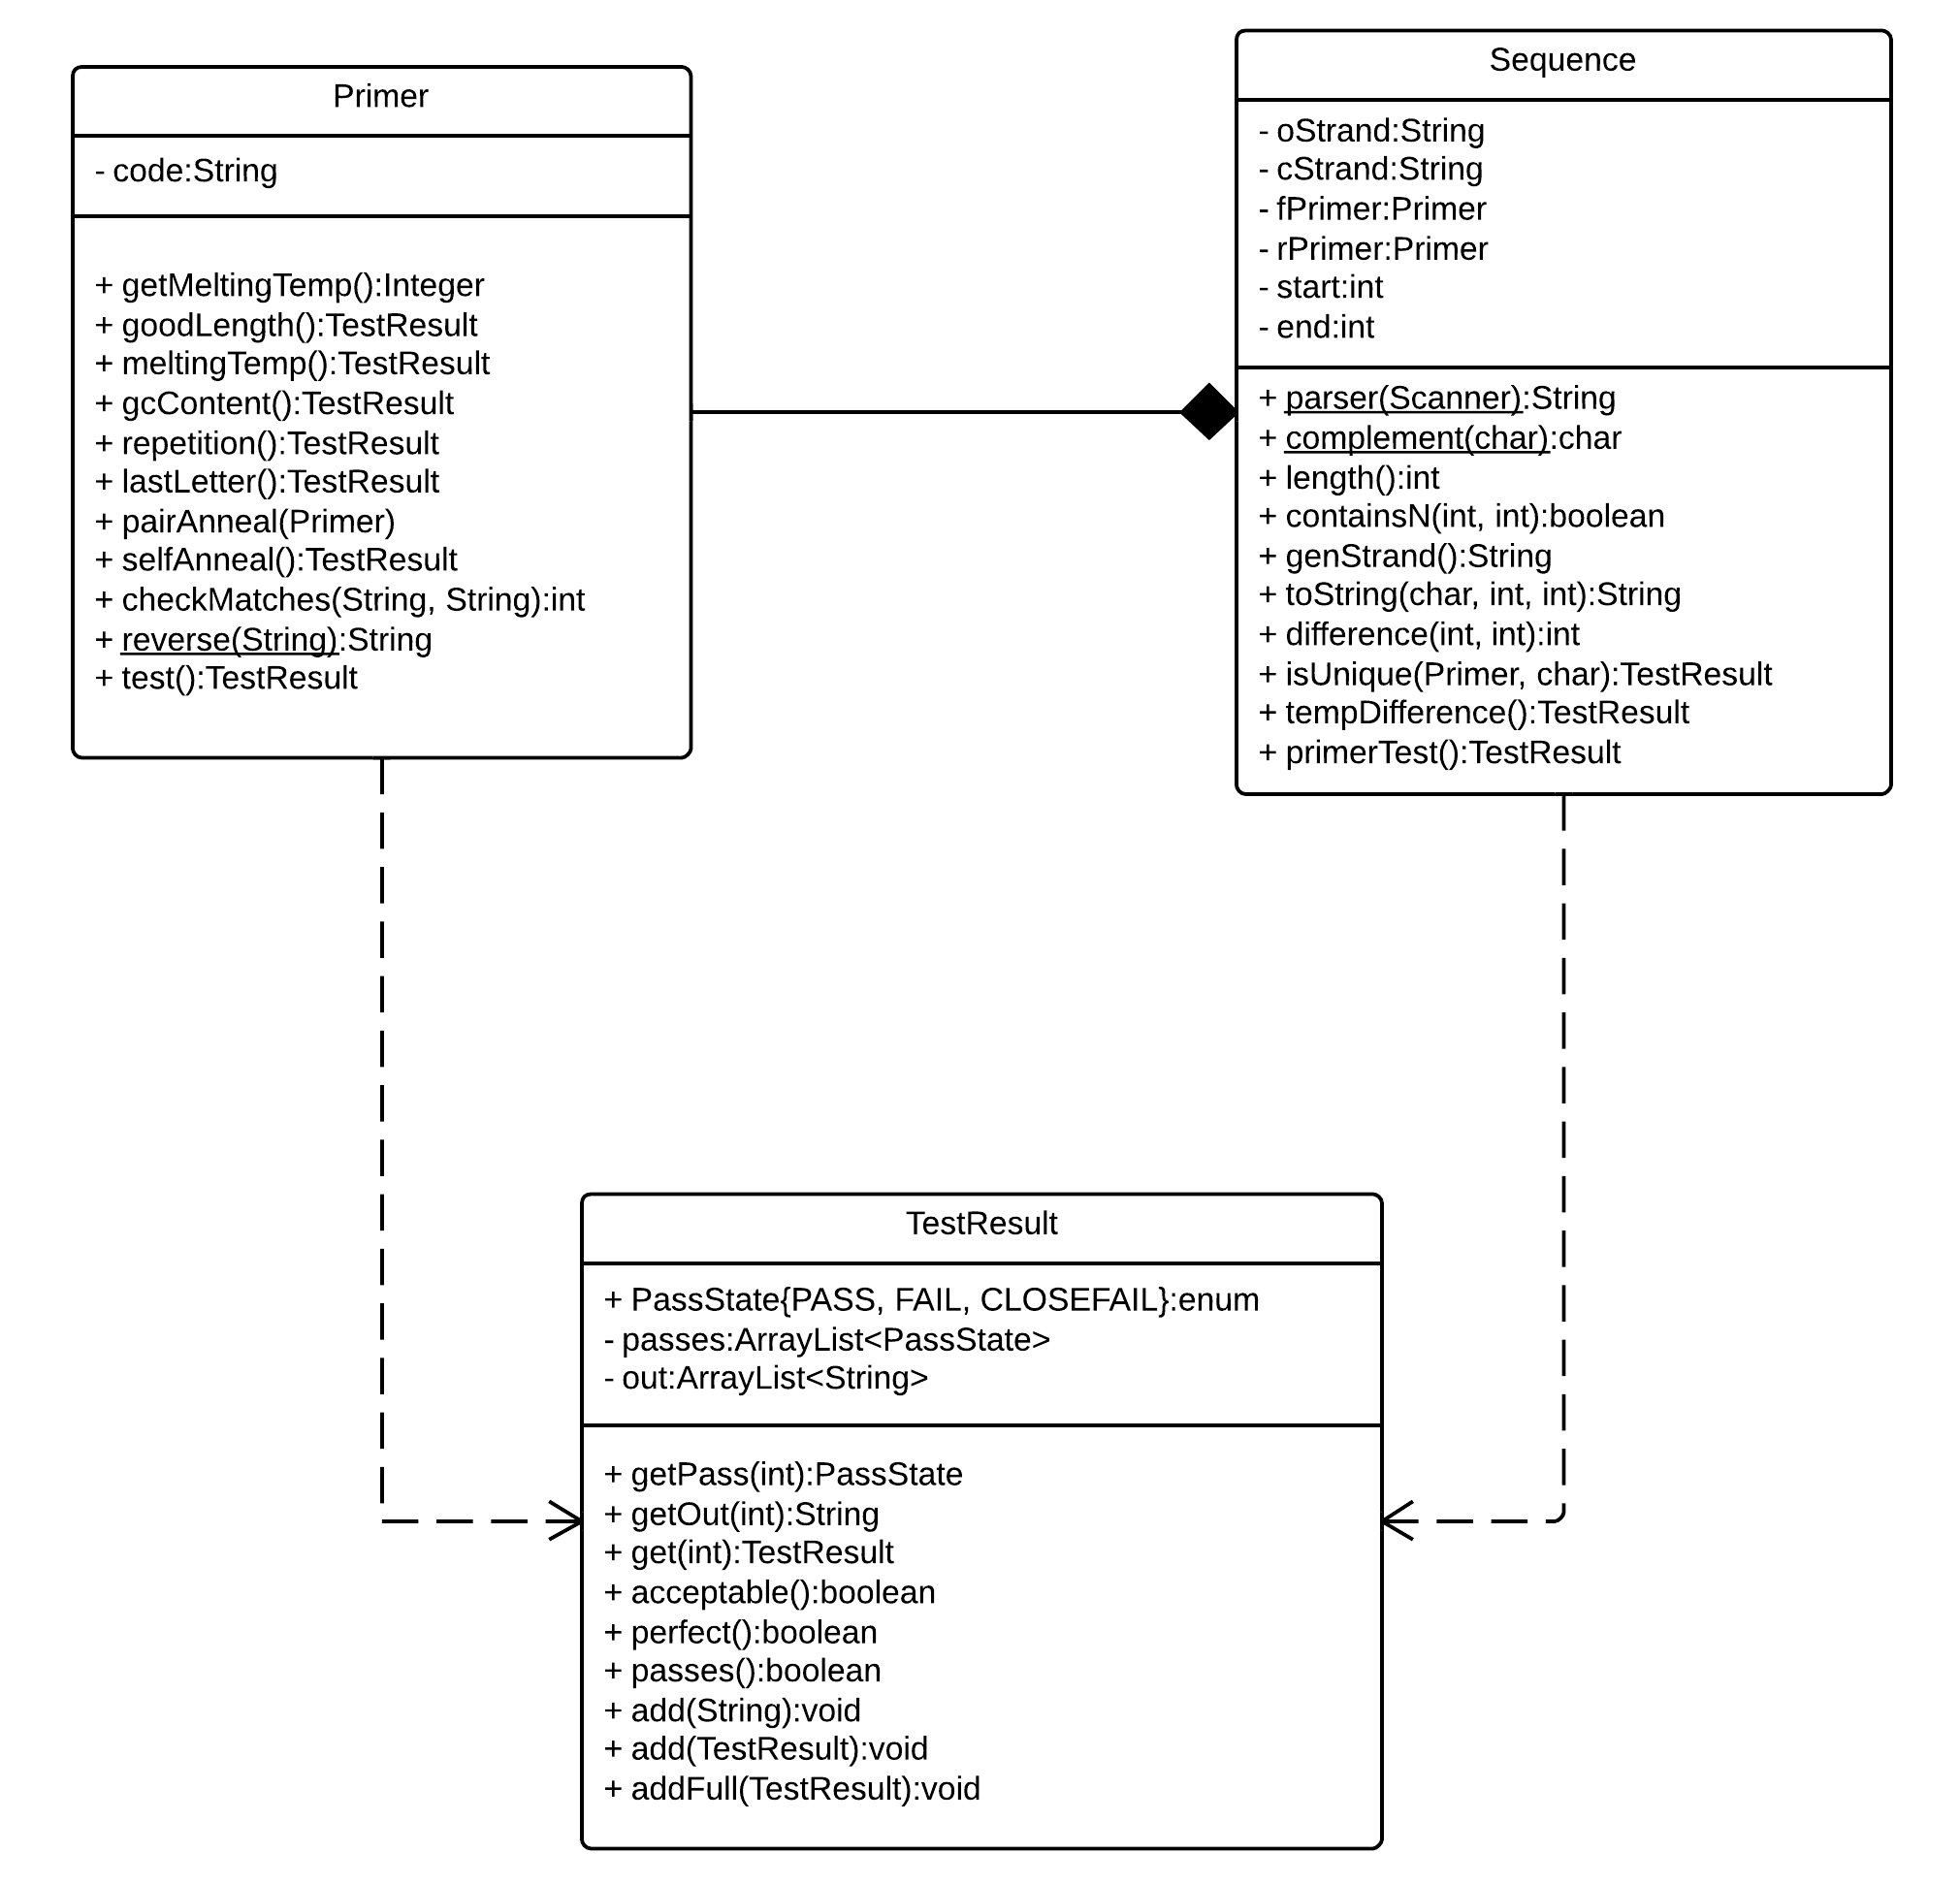
\includegraphics[width=0.75\textwidth]{./images/currentBuild/modelClassDiagram.png}
    \caption{
      \label{fig:currentBuild:model}
      Model Class Diagram 
    }
  \end{center}
\end{figure}

The models used in the application are few in number and do not have complex relationships
with each other (as can be seen in Figure \ref{fig:currentBuild:model}), as we strove to 
keep the structure as simple as possible in the interest of runtime efficiency and a clear
design.

As seen in Figure \ref{fig:currentBuild:model}, we used three classes to represent the data:
Primer, TestResult and Sequence.

\paragraph{Primer}
The Primer class is purely designed to test user-designed primers. It has 
one instance variable, \texttt{code}, the String representing a primer
which is tested against the primer test methods, which make up the 
remainder of the class. The class is primarily made up of methods 
designed to test \texttt{code} against the various rules described in Section 
\ref{intro:prelims}. The method \texttt{test()} runs all above test 
methods and returns a TestResult indicating if the user's Primer 
is adequate without testing it against the opposing primer or its position
in the sequence as a whole.

\paragraph{TestResult}
TestResult is a class used to format the output of one or multiple primer 
tests. TestResult uses an enumerated type called PassState with values
\texttt{PASS}, \texttt{FAIL} and \texttt{CLOSEFAIL}, the last of which describes 
a state where the primer's value from a test lies outside of the recommended
values, but is within 10\% of a pass (in all tests with numerical boundaries) 
and as such is seen as acceptable, provided this is 
only the state of a minority of tests. TestResult uses two ArrayLists, one of
PassStates (\texttt{passes}) and another of Strings (\texttt{out}), to keep track 
of the state and informative message to be displayed to the user for each 
test. 

Its methods are concerned with concatenating results into larger 
TestResults. \texttt{perfect()} will return true if all entries in 
\texttt{passes} equal a \texttt{PASS}. \texttt{adequate()} will return true if the
primer follows a requisite number of general design rules (60\%) to function 
sufficiently, and is checked when deciding if a user can progress past the
primer selection stage of the exercise.
 
\paragraph{Sequence}
This class contains two Strings, \texttt{oStrand} and \texttt{cStrand}, 
representing the strand of DNA that the user entered and the ''complementary''
strand that is generated by the \texttt{parser()} method (described below)
when the sequence is constructed. Integers \texttt{start} and \texttt{end} represent 
the indexes of the start and end of the selected area in the sequence, and Primers 
\texttt{fPrimer} and \texttt{rPrimer} are representations of the user's forward
and reverse primers, respectively.
 
\texttt{parser()} is used for both sequence entry and primer input, by taking in
a String and returning a new String with all non-\texttt{atgc} characters removed.
This is due to the formatting of the NCBI page, which includes line numbers that
would interrupt the sequence.
\texttt{complement()} is a very simple function used throughout the application
that takes in one character representing a base, and returns its complement, i.e.
\texttt{complement('a')} would return \texttt{t}. \texttt{isUnique()} and \texttt{
tempDifference()} check the user's primers against their place in the larger sequence
and the difference in their temperatures. \texttt{primerTest()} uses all other test 
methods to return a TestResult that will ultimately decide if the user's primer is
adequate.  																										% phrasing?


\subsection{Primer Checking}
The `Primer Checks' methods are implementations of the established rules
and guidelines which are used in the process of Primer Design (seen in
Section \ref{intro:prelims}) to evaluate the effectiveness of a given 
Primer when used in the PCR process.

As with many other aspects of the project, the primer checks were split
between the two members of the 'back-end' sub-team. As well as making
this task more manageable, this approach offered the added benefit of
limiting the researching of primer design rules to two members, who each
only had to learn how to apply the rules assigned to them.

The implementation of these rules varied widely in difficulty, from
trivial checks such as ``Primers should end in a base \verb£g£ or \verb£c£'' 
to more challenging problems such as checking how likely it is that a primer  
will self-anneal.

Firstly, as discussed in Section \ref{intro:motiv} none of the members of 
the team had any experience with PCR or Primer Design prior to the start of 
the project, and so every rule had to be thoroughly studied and understood 
before design of the methods could begin. However, even after spending time 
learning how the design rules and guidelines are used, some methods still 
proved problematic.

\subsubsection{Melting Temperature}
The melting temperature check was among the easiest to implement, as we
were given a standard formula for calculating the temperature at which a 
primer would melt (\texttt{2*sum(a, t) + 4*sum(a, t)}) and the desired 
range in which a primer should rest (between roughly 50\degree C and 
60\degree C).

\subsubsection{Uniqueness}
To check that the primer is correctly placed in the system, it is first checked
that the primer cannot be found in the wrong strand (ie. that the forward
primer cannot be found on the complementary strand). When this is confirmed,
it is then checked that the correct strand contains one and only one instance
of the primer, and then that this instance is positioned correctly, relative
to the area of the sequence to be replicated.

\subsubsection{Primer Content}
Many of the primer rules were trivial to implement in the system, given
the string representation of a primer. Such rules include ensuring the
length of the primer lies between 20 and 30 bases, checking the last base
of a primer and confirming that no base is repeated more than 4 times
in a row. 

\subsubsection{Annealing}

As mentioned in Section \ref{intro:prelims}, there is an increased
chance of primer annealing happening if it is possible for a pair of
primers (or a single primer folding over on itself) to line up in such a
way as to produce 4 or more consecutive complementary bases between the
primers (or the two sections of a folded over primer). To aid with the
implementation of both the Self Annealing check and the Pair Annealing
check a function called \texttt{checkMatches()} was created. This function
takes in two primer subsequences (as strings) and returns the highest 
number of consecutive complementary bases in the two sequences.

\subsubsection{Self Annealing}

As described above, our \texttt{checkMatches} function compares
complementary bases between two strings. Therefore, to use this function
to check for annealing between two ends of a single primer the primer
has to be split into two strings. To keep track of the index where the
primer has been split there is a variable, \texttt{split}.

The main body of the function is a while loop which calls
\texttt{checkMatches()} on the two sections of the primer which are
separated by \texttt{split} then increments \texttt{split} and if loops
again if \texttt{split} is at least 4 positions away from the end of the
primer. During this process the highest result from the
\texttt{checkMatches()} calls is recorded and this is used to determine
wether or not the primer is likely to self-anneal.

\subsubsection{Pair Annealing}

This function works in a similar fashion to the Self Anneal checking
method in that it compares the two primers in every possible alignment
and stores the highest number of matches.

The difference here is how the strings which are sent to the
\texttt{checkMatches()} function are selected. In the
\texttt{pairAnneal()} function this is done in three separate while
loops. The first while loop checks all possible alignments when the
shorter primer overlaps the longer one at the start, for example:
\begin{verbatim}
       agtcatcg
    acatca
\end{verbatim}
The second while loop checks the alignments when the shorter primer does
not overlap either end of the longer primer, for example:
\begin{verbatim}
     agatcgattgcagt
        agctaac
\end{verbatim}
And the third while loop checks the alignments when the shorter primer
overlaps the longer primer at the end:
\begin{verbatim}
     agtacgtaggtc
            tccagtac
\end{verbatim}
Once every possible alignment has been checked, the function uses the
highest number of matches to evaluate the likelyhood of the primers
annealing to each other.















\subsection{Dynamic Primer Highlighting}

Dynamic Primer Highlighting was suggested early on in the requirements
elicitation process by the clients as something that would be very
helpful to students studying primer design. The initial specification
for this feature was as follows:

\begin{itemize}	
\item“As the user enters their choice of primer in one of the boxes at the
top of the page, instances of the primer should be highlighted in
real-time in the corresponding box below containing the DNA sequence for
the strand on which this primer should appear.”
\end{itemize}

In a later client meeting the following addition was made to improve the
effectiveness of the feature:

\begin{itemize}
\item“Primers should be highlighted in different colours to indicate their
suitability.”
\end{itemize}

This was a feature that all members of the team appreciated from a very early
stage because, even with our limited knowledge about primer design we
could see how this form of immediate feedback had the potential to
improve the usability of the system if it were to be implemented well.
Due to this level of popularity among both the clients and the team
members the feature was given high priority. However, since we knew it
would be complex to implement and would require calls to other planned
modules of the system, such as the primer checking functions, it was
also decided that this should be one of the last features to be
implement.

This feature turned out to be one of the most problematic features to
implement as it involved using features of Java which we had no real
experience with, specifically the Swing classes
\texttt{Change\-Listener}, \texttt{Highlighter} and \texttt{Painter} as
well as integrating other modules of our code to provide the required
primer checking. This level of difficulty meant that this feature
actually took multiple attempts to implement correctly.

\subsubsection{Implementation}

The implementation of this feature can be split into two main
components:

\begin{itemize}
\item The code to listen for user input in the primer entry text fields
and call the appropriate methods to deal with the input.
\item The runnable objects \texttt{searchO} and \texttt{searchC} which
are called by the listener and update the highlighted text.
\end{itemize}

\subsubsection{Listening for Input}

The first challenge when implementing this feature was deciding how to
listen for user input in the \texttt{forwardPrimerTextField} and
\texttt{reversePrimerTextField}.

Due to the fact that only one strand's display tab would be shown at any
given time, only the TextField related to the active tab would have to
be listened to and any user input in the other field could be ignored
until the active tab changed. This meant that only one listener would be
needed and the TextField it was listening for updates on could be
switched when required.

Since this feature was implemented late on in the development cycle,
code already existed to deal with changes upon switching tabs.
Therefore, we were able to add the calls to switch the TextField being
listened to into the existing \texttt{updateLineNums()} function which
was only being used to update the line numbers upon switching between
single and double-stranded views.

As well as switching the target of the listener upon switching tabs, a
call must be made to the search function related to the new tab since
any user input into the corresponding TextField while the tab was not
active will not yet be reflected in the display tab. This call is made
using the \texttt{invokeLater()} call of the runnable search function
as oppposed to a standard \texttt{invoke()} call to allow the system
to continue listening for updates if a call to one of the search
functions takes a long time to process.

Once we had worked out how we were going to switch the listener focus
all that was left to do in terms of listening for input was to add code
to the \texttt{DocumentListener} functions
\texttt{insert\-Update()} and \texttt{removeUpdate()} to run the
appropriate search function. This just required an if statement to
determine the source of the update and inside the if statement a call to
the appropriate search.

\subsubsection{Runnable Search Functions}

After dealing with listening for user input, the next task was to create
the functions to search for the user's primer in the DNA sequence and
highlight the appropriate sections.

To perform this task we created two similar methods: \texttt{searchO()}
to search the parsed version of the strand entered by the user,
\texttt{parsedO}, and update forward primer highlights and
\texttt{searchC()} to search the parsed complementary strand,
\texttt{parsedC}, and update reverse primer highlights. 

The first task these functions perform is removing all existing
highlights from the display. The other option here was to keep a list of
all highlights and their positions in the sequence then check each one
individually to determine if they were still valid after the latest
input and highlight an extra base at the start of end of the old
highlight. This list based solution was not chosen because, for example,
if a user's first input was a single letter then the program would
potentially have to store the positions of thousands of bases and
perform thousands of comparisons on their next input.

The next step is to get the position of the first instance of the primer
in the sequence using the Java \texttt{indexOf()} function, which returns
the index of one String within another. This is then
used as part of the condition of the while loop which carries out most
of the functionality in these methods. The while loop is executed while
the result of the \texttt{indexOf()} call is not negative (i.e. the
primer is found in the text being searched) and the user input has a
length greater than 0 (i.e. the call to the function was not because the
user deleted everything in the text field).

Inside the while loop the colour of the current instance's highlight is
determined by the following if statement from \texttt{searchC}:

\begin{verbatim}
    if (sC.length() > 15){
        Primer rPrimer = new Primer(Primer.reverse(sC));
        rTest = new model.TestResult();
        rTest.addFull(rPrimer.test());
        rTest.add(
            rPrimer.isUnique(PrimerDesign.start.getInSequence(),
                'c'));
        if (rTest.perfect()){
            activePaint = perfectPaint;
        } else if (rTest.acceptable()){
            activePaint = acceptPaint;
        } else {
            activePaint = failPaint;
        }
    } else {
        activePaint = failPaint;
    } 
\end{verbatim}

Here, \texttt{sC} is the user's primer input and \texttt{perfectPaint},
\texttt{acceptPaint} and \texttt{failPaint} are different coloured
\texttt{Painter} objects initialised when \texttt{PrimerSelectionPanel}
is first loaded. The only difference between the three \texttt{Painter}
objects is their colour with \texttt{perfectPaint} being blue,
\texttt{acceptPaint} being yellow and \texttt{failPaint} being red.
These were initially green, yellow and red but green was eventually
substituted for cyan due to concerns about colour-blind users.

The late stage at which this feature was implemented meant that the
process of evaluating the user's primer was a trivial task as all the
methods which check the primer were already written, as were the methods to
evaluate the success of the primer overall. So the method simply has to
create a new \texttt{Primer} instance with the user's input and create
an instance of \texttt{TestResult} to store the results of the primer
checking methods. Then the method calls the \texttt{perfect()} and
\texttt{acceptable()} methods to determine the colour the primer should
be highlighted.

Once the colour of highlight has been determined the highlight is
applied to the correct section of the DNA sequence using the following
code:

\begin{verbatim}
    endC = indexC + sC.length();
    highC.addHighlight(realIndex(indexC + checked, 10),
        realIndex(endC + checked, 10), activePaint);
\end{verbatim}

\texttt{endC} is calculated by adding the length of the user's primer to
the index of the current instance of the primer in the sequence, 
\texttt{indexC}. \texttt{realIndex} is a function which converts the
indices in the parsed sequence into the indices needed for displaying
the highlights in the display panes.

Once the current instance of the primer has been highlighted, a 
\texttt{substring()} is performed on the relevant parsed sequence to
remove everything up to the end of the current primer instance. The
index of the first instance of the primer in this new, shorter sequence
is then found and if this index is greater than or equal to 0 then the
while executes again to highlight this new instance of the primer. This
is less than ideal, as it precludes the detection of matches that begin
inside another match, however we are committed to finding a solution to
this problem in our future work, as discussed in Section \ref{eval:future}.



After all instances have been highlighted the parsed sequence is reset
to the state it was in before the function was called.













\subsection{Other Methods}

\section{Animation}
\label{impl:anim}
\paragraph{Required Functionality}
Our initial plans for the animation were to make it depend on the actual user input in the exercise itself, particularly taking the sequence and the primers from the previous stages of the application. This was mainly to differentiate more from other similar PCR animations, like those demonstrated to us by the clients (see Section \ref{intro:motiv}. Because of the high customisation requirements set by the task at hand and to provide maximum compatibility throughout the project we decided to develop the animation on Java utilising Java graphics package and Swing together, with the animation logic being developed from scratch. However, towards the end of the animation development it became apparent that the sequence required to be presented in the animation is just too large to be reasonably scaled with the individual bases being visible. To extrapolate, the individual bases were hard to make out as soon as the target PCR area reached about 150 bases in length, which was not enough as the area could be well over that limit. Finally, as the clients were satisfied with a static animation, it was decided that we would just use the animation with a sample input that  was adequately sized. It was also suggested by the clients that the individual base's colour coding doesn't need to be explained in the animation as it was clear enough that the different colours represent different bases. Otherwise the aforementioned shift in the overarching animation design didn't affect it in any way. The final animation sreenshots and explanation of its individual parts are provided below.

\paragraph{Implementation}
The whole animation is controlled with a large set of conditional statements by a Swing timer that constantly recalculates the time passed from the start of the animation, pausing if it reaches the end of a stage until a button press changes the stage and therefore sets the time passed to a particular value. The models used in the animation were developed in the Inkscape vector graphics editor and are the different type of the individual base's models, the Taq polymerase model and three models for three different states of the thermometer. The individual bases are then drawn to make a sequence at a particular location.

\paragraph{Functionality Explained}
The animation is split into 7 stages, each with a related explanatory statement at the bottom. A thermometer is displayed at all times on the screen to show the current temperature at each stage of the process. Four buttons lie above the descriptive text: ``Close", to close the application completely; ``Restart", to go to the start of the exercise; ``Previous" and ``Next" to navigate between the animation stages. The animation won't proceed until the ``Next" button is pressed, something which was suggested by the clients, as they pointed out that the user might not be able to read the text in the time provided. Finally, the PCR animation itself is in the top part of the screen.

\paragraph{Animation Screens}

In the stages 0 and 1, PCR is briefly explained in simple terms as the temperature rises to 72\degree C.

\begin{figure}[h]
  \begin{center}
	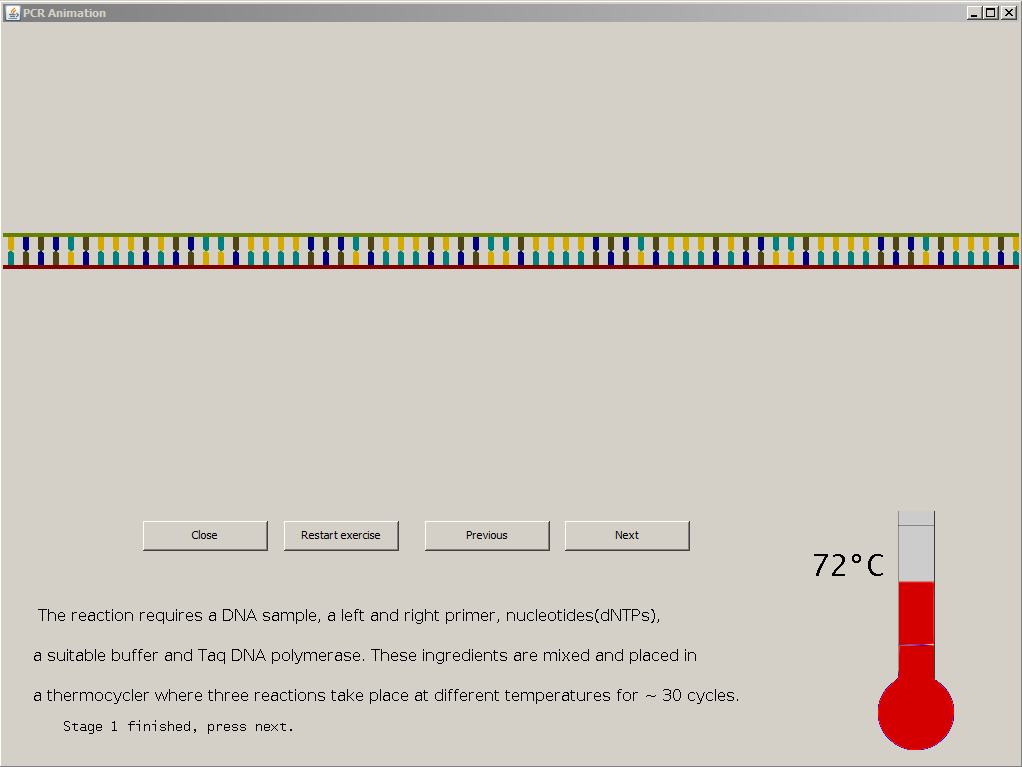
\includegraphics[width=0.6\textwidth]{./images/AnimImpl/Stage1.png}
    \caption{
      \label{fig:AnimImpl:stage1}
      Animation, Stage 1
    }
  \end{center}
\end{figure}


In stage 2, Melting and Annealing, the strands are separated and the primers bind to them, with the temperature level varying accordingly.

\begin{figure}[!t]
  \begin{center}
	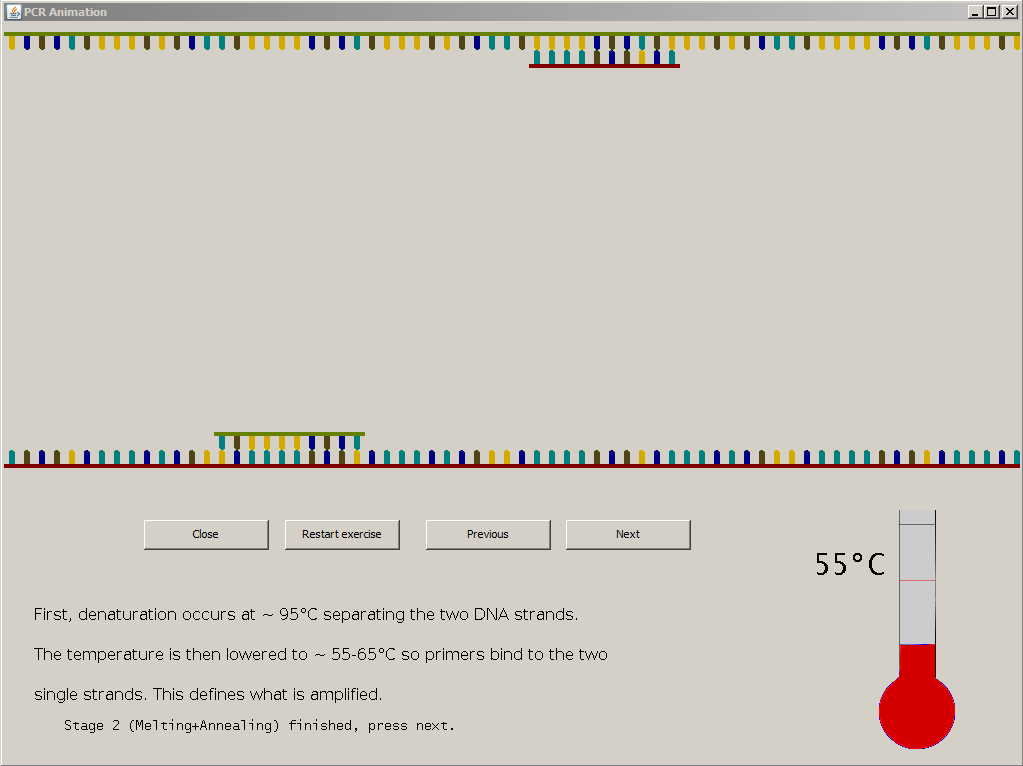
\includegraphics[width=0.6\textwidth]{./images/AnimImpl/Stage2.png}
    \caption{
      \label{fig:AnimImpl:stage2}
      Animation, Stage 2
    }
  \end{center}
\end{figure}

In stage 3, Adding nucleotides, the taq polymerase creates a complementary copy of each strand, with the temperature once again raised to 72\degree C.

\begin{figure}[!t]
  \begin{center}
	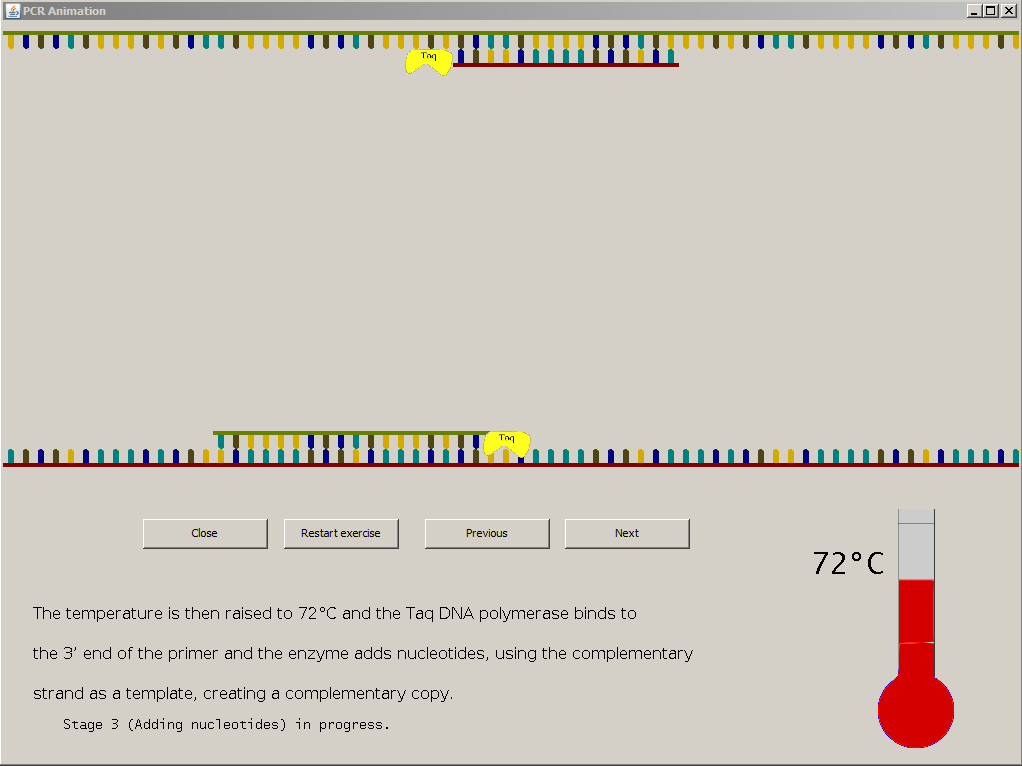
\includegraphics[width=0.6\textwidth]{./images/AnimImpl/Stage3.png}
    \caption{
      \label{fig:AnimImpl:stage3}
      Animation, Stage 3
    }
  \end{center}
\end{figure}

In stages 4 and 5 another cycle of PCR is shown and the required sequence is generated for the first time.

\begin{figure}[!t]
  \begin{center}
	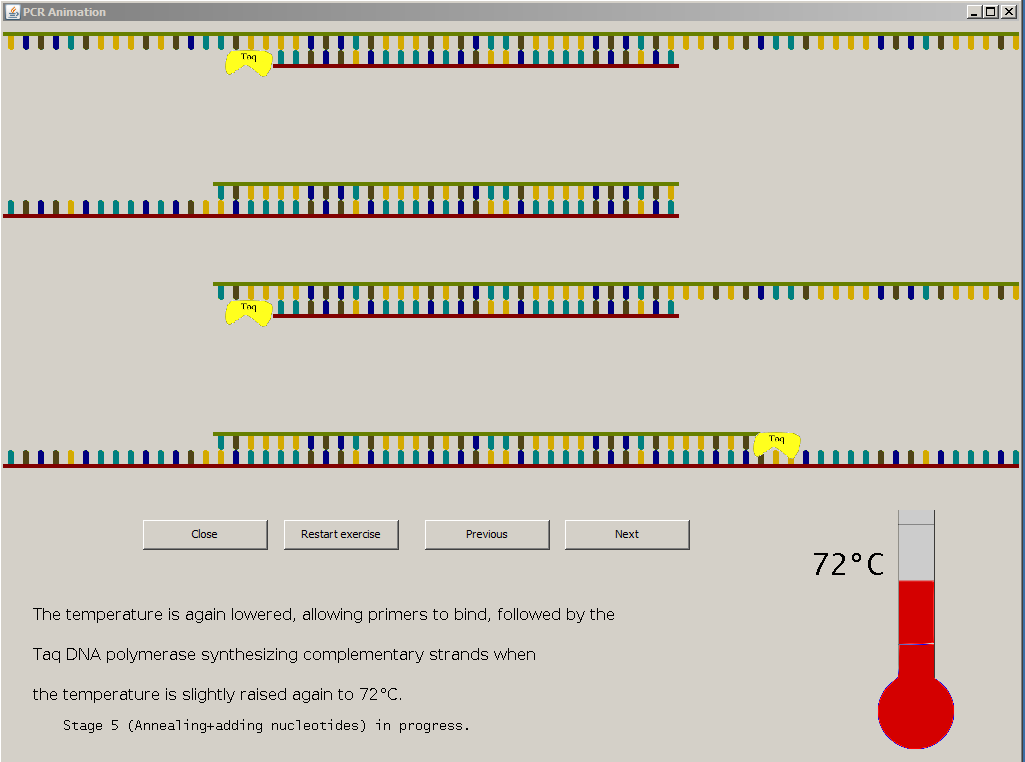
\includegraphics[width=0.6\textwidth]{./images/AnimImpl/Stage5.png}
    \caption{
      \label{fig:AnimImpl:stage5}
      Animation, Stage 5
    }
  \end{center}
\end{figure}

Finally, the last two stages explain how many copies of the target sequence is produced in subsequent cycles and the user is explained that they completed the exercise and thanked for participation.

\begin{figure}[!t]
  \begin{center}
	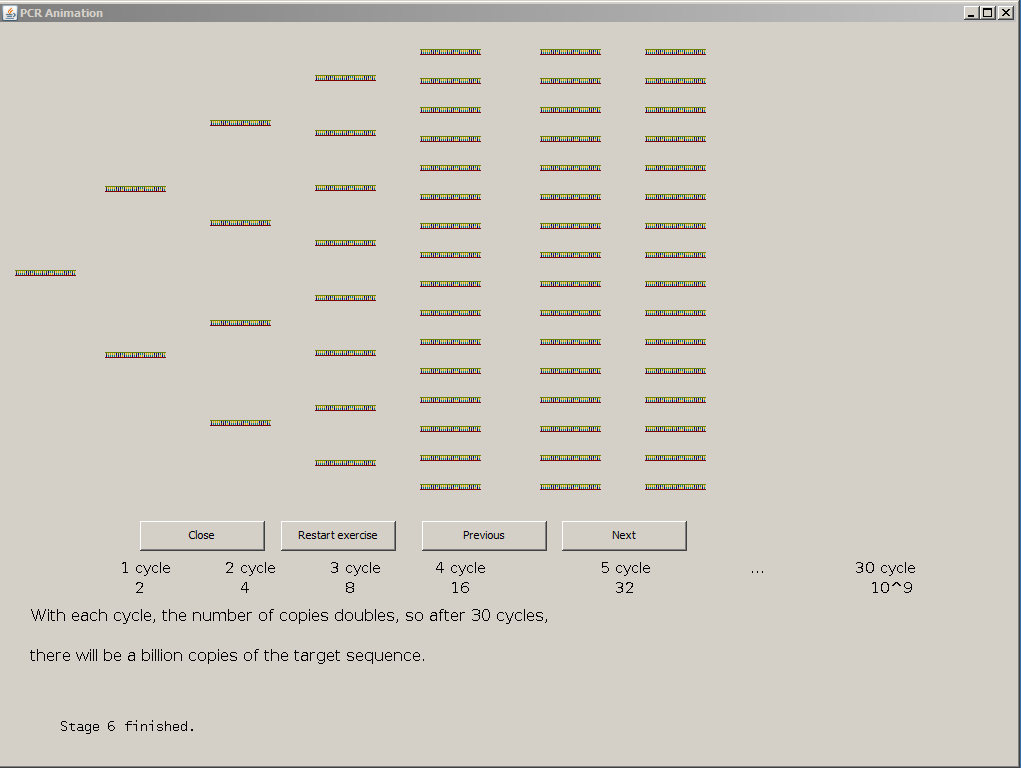
\includegraphics[width=0.6\textwidth]{./images/AnimImpl/Stage6.png}
    \caption{
      \label{fig:AnimImpl:stage6}
      Animation, Stage 6
    }
  \end{center}
\end{figure}


%=====================================================================
\chapter{Evaluation}
\label{eval}

\section{Testing}
\label{eval:testing}
% ADD TO THESE COMMENTS AS YOU SEE FIT 
%
% Testing - Internal Testing, give to the supervisors for feedback, changed according to their requirements
%
% Demo - dry run through with students. Given user guide and feedback sheets, changed according to their feedback
%
% Questionnaire - Sent out with jar file on moodle, feedback from students on 'finished' application
\section{Introduction to Testing}

As with any software development, testing is a necessary component. During our time with the PCR application, testing begun
almost as soon as implementation started. Our testing fell into two categories: \\

\begin{itemize}
\item Testing of the backend, such as primer checking formulas etc.
\item Testing of the user interface.
\end{itemize}

Also, with reference to the (edit ME)\cite{Lethbridge}, we accomodated for both white and black box testing. 

\subsection{White Box Testing}
White box testing was
used throughout the development of the implementation, as we all had an indepth knoweledge of the source code. This enabled us to test
for defects by creating scenarios which tested the programs to its limits and beyond, in order for us to assur






\subsection{Demonstration}
On the 8th February, our team carried out a demonstration run of our software with a group of users connected to the School of Life Sciences. In this test, we provided users with a comprehensive user guide and asked them to carry out a set of tasks using, what we called at the time, the demo build of the application. With this version of the program we had decided to disable the animation, as the animation had been developed using Java 7 \cite{Java7SwingAPI}, whereas the rest of the application had been developed using netbeans and Java 6, as had been decided before implementation, (See: chapter \ref{chap:impl}). However, the rest of the application we believed to be functioning at the time of the demo run, minus some major features we had yet to implement, such as the dynamic highlighting feature implemented in the final version (See: Section \ref{impl:models:dynHigh}).

\subsection{Running the demonstration}

The demonstration took place between 12pm and 1pm in a computer lab in the Wolfson building, with a group of about 12 participants, consisting of students, demonstrators, lecturers, and the clients. The computers on which the application was run were all identical, all running on Windows 2000. We issued each participant with a user guide (See related documentation), detailing how to load the application from moodle and get it running, and then gave them clear instructions as to how to use the application to test for correct primers. Three members of our team (Ross Eric Barnie, Murray Ross and Ross Taylor) were on hand to help participants with any problems they may have had with the program. We let them work with the application for about half an hour before asking them to finish their work and sit down to have a round table discussion about their experiences with the system, and to fill out an evaluation sheet which we also provided them with.

\subsection{Feedback from demonstration}

At the round table discussion, we used a sound capturing device to record what people had to say about the application, which was later annotated in a text document (See: Appendix \ref{app:roundtableFeedback}). Also, we asked participants to fill out an evaluation feedback sheet at the end which was then read by our team and the points were collated and annotated into another text document (See: Appendix \ref{app:demonstrationFeedback}). The main points that were taken from the feedback provided by the demonstration were:

\begin{itemize}

\item That the primer rules were unbreakable - you could not progress to the melting temperature screen without passing all the rules set by the program. In a typical DNA sequence, finding a 'perfect' primer is extremely hard, and the rules should be there more as guidance, not as set in stone.
\item Further to the first point, using the words 'PASS/FAIL' is too harsh, and the capitalisation should be taken out.
\item That the interface shown to the participants that whilst clear, was very clinical, very '90s'.
\item As a teaching tool, the application was definitely better than any paper version previously provided by the School of Life Sciences.
\item The purpose of the application was misconstrued - it isn't there to find primers for you, it is there for the user to find them and test them.
\item It would be helpful if the program could check each primer individually, and not together at the same time.
\item The application required the user to use keyboard shortcuts to copy/paste, and that a few participants did not use these shortcuts in common use and preferred graphical buttons to do these functions.
\end{itemize}

We then collected in the evaluation feedback sheets from the participants. The main points that we took from these sheets were:

\begin{itemize}

\item In general, it was always clear how to progress in the application from stage to the next.
\item Aesthetically, the application did not have a ostentatious design but it met the demands and expectations of the user.
\item The rules provided in the \emph{Primer Design Rules box} were very helpful, but should point out these are only guidelines and not set in stone.
\item If you infringed on a rule, it should allow you to pass through anyway, perhaps using an \emph{override} button.
\item Some users found it to improve their knowledge of primer design.
\item It was noted that if you had a higher melting temperature in your first primer (i.e. 64) than the second (i.e. 62), but both were still in the melting temperature range, it would tell you that they were not within the required temperature range of each other, yet they clearly were.
\item Reverse primers would dissapear from screen, forcing users to write them down if they wanted to remember them.
\item A helpful idea would be that as the user entered their primer it highlighted it on the sequence for them to see.

\end{itemize}

With this feedback, we were able to decide on which changes were required to the program.

\subsection{Changes proposed after feedback from demonstration} 

After we had met to discuss the feedback, the following changes to the application were decided upon:

\begin{itemize}

\item Implementation of the dynamic highlighting feature (See: Section \ref{impl:models:dynHigh}) - whilst this was initially our intention during development, we had failed to implement it in time for the demo. However, from the feedback above where users were losing their primers during usage of the application, and also for general accessibility purposes, we decided implementing this feature had become a priority.

\item Reduce the strictness of the primer design rules. From the feedback we received above, we found that users had previously used these rules as guidelines to follow in primer design, and that they were not necessarily adhered to all the time. Therefore, we decided that instead of requiring a 100\% success rate in order to reach the melting temperature screen, we would allow users to 'override' the rules after 3 attempts, making the rules more like the guidelines users were expecting as opposed to set in stone.

\item After users had notified us of the bug which tells a user that their temperatures were not in range when they were, we decided to analyse the formula for calculating the temperature in order to fix this fault.

\item Some users had noted in the roundtable discussion that they would like to be able to check each primer individually, as opposed to both at the same time. To accommodate this, we decided to implement individual primer checker buttons on the primer selection panel to allow users to check each primer separately against the guidelines.

\item Certain users were confused by the lack of copy/paste buttons on the user interface, and did not know the keyboard shortcuts to use in order to get around this. To allow users more accessibility, we decided to implement graphical buttons for copy/paste.

\item The feedback we received indicated that they though the program was too harsh and clinical when it came to notifying users of their test results for their chosen primers. To help this, we decided to replace capital letters in the pass/fail messages to reduce harshness.

\end{itemize}

\label{eval:demo}

\subsection{Questionnaire}
\label{eval:question}
In order to test the final system against the requirements set out in
section \ref{design:reqs}, the team decided to produce a
questionnaire which would be given to students using the application
for them to give us feedback.
The raw data for this feedback is shown in appendix
\ref{app:questionnaireResponses}.

While other methods of testing exist (e.g. experimental) it was felt
that with the time constraints in place we would not be able to run a
test requiring our direct involvement and that we would receive more
data from a questionnaire.

%---------------------------------------------------------------------
\subsection{Questionnaire System}

Many questionnaire services exist on the internet, such as
SurveyMonkey \cite{surveyMonkey}, FreeOnlineSurveys
\cite{freeOnlineSurveys}, and Google Docs Forms
\cite{googleDocsForms}.

The team decided to use the Google Form, simply because most members
of the team have a Google account, and because it was free.

On closer inspection it could also export its responses to a Google
Docs Spreadsheet which itself could be exported to a variety of
formats.

%---------------------------------------------------------------------
\subsection{Questions}

Generally, the questionnaire needed to be as concise as possible to
avoid any data being corrupted by frustration at the questionnaire.
To this end we kept the number of questions in general to a minimum
and only asked for a description if it was necessary.

\subsubsection{Skill Level}
At the demonstration, the team realised that not every user will be in
the expected age bracket of 18 to 20-years-old who have used computers
their entire lives.
This led to the decision that the feedback should take the user's age
into account, to ensure that there are no patterns in the data
suggesting a particular age group struggles with the application.

In addition, we ask the user for their ``Confidence'' with computers
in general, on a scale from 0 to 5 ie no middle option so there has
to be a bias to confident or not confident.
This completely subjective question should allow us to see if people
who perhaps do not use computers on a daily basis handle the
application, since we believe we made the application (and
accompanying user guide in appendix \ref{app:userGuideCurrent}) as
user-friendly as possible.

We are also aware of some colour-use in the program that could be
problamatic for colour-blind people so we ask the user if they are or
not.

To get an idea of the user's knowledge of primer design, we ask the
user for their self-assessed understanding before using the system, on
a 0 to 5 scale.

All of this data provides us with the baseline skill level with
computers and with primer design of the user, before they use the
system.

\subsubsection{User's Experience with the System}
The following questions were designed to provide us with feedback on
the user's experience with the system.

The first of these follows the self-assessed understanding of primer
design before using the system, with a self-assessed understanding
after using the system, on the same scale.
This will provide us with test data towards the requirement to teach
students about primer design and PCR.

Ideally, as discussed in section \ref{design:reqs}, the system would
be used as a revision tool in students' own time and/or in a
laboratory setting with tutors on hand to help the student with any
problems.
To see if we met this requirement, we asked the user if they would use
the system to study one of the following options:
\begin{itemize}
\item Both Primer Design and PCR
\item Just Primer Design
\item Just PCR
\item Neither
\end{itemize}
Which provides the user, and the team, with every possible answer to
the question, in the most concise way possible.

Following this, we decided to ask the user if they felt they were
given enough information from the application.
In retrospect, this question should have been clearer in that it
should have specified to disregard the user guide.
We wanted to ask this to assess how easily people would be able to use
the application without the user guide.

Technical difficulties were fairly common in the demo build (section
\ref{eval:demo}) but since members of the team were present, we could
instantly know about them.
However since the system was now being used from where the user
happened to be, we had no direct way to be told of any technical
issues or bugs.
To this end, we asked the user for any technical issues they found
while using the application.

Lastly, we ask for any further comments, in case the user wanted to
tell us something we had not asked before this point in the
questionnaire.
To keep it light-hearted, we recommended telling us a joke in the
description of the question, needless to say we had some interesting
feedback for this particular question.

%---------------------------------------------------------------------
\subsection{Feedback Analysis}

In total we received 15 responses, see appendix
\ref{app:questionnaireResponses} for the raw data.
These responses have yielded some interesting results with a few
anomalies.

\subsubsection{Learning}

Of course, the main objective of the system is to help users revise or
solidify the idea of primer design within PCR, if we have not managed
this, we have failed our users.

\begin{figure}[h]
  \begin{center}
    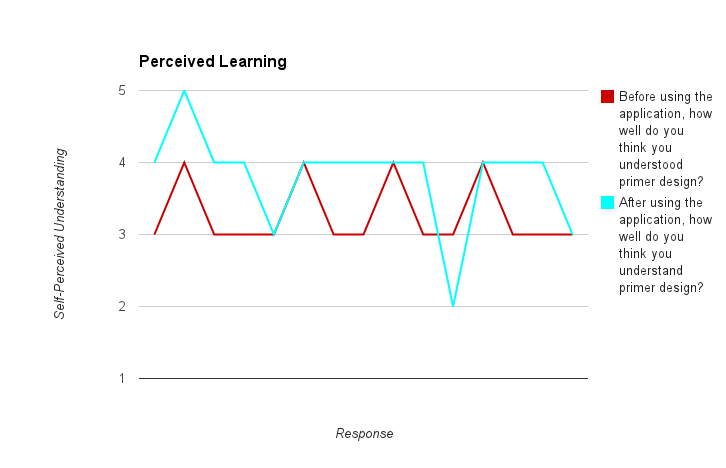
\includegraphics[width=\textwidth]{./images/perceivedLearning.png}
    \caption{Perceived Learning Chart}
    \label{fig:feedbackAnalysis:perceivedLearning}
  \end{center}
\end{figure}

If the application was perfect in this regard and a graph was plotted
for response against score given to the ``Before'' and ``After''
understanding questions, the graph would show that the ``After''
responses line was consistently above the ``Before'' line, implying
that users always see an improvement in understanding.
Unfortunately, as can be seen in figure
\ref{fig:feedbackAnalysis:perceivedLearning} which used the data in
appendix \ref{app:questionnaireResponses}, this is currently not the
case.

One third of responses stated that their understanding of primer
design stayed the same before and after using the system and, more
concerningly, one response claimed that using the system reduced their
understanding.
This still means that a majority of users, 60\% of users who responded
to the questionnaire, found using the system increased their
understanding, however this still implies that 40\% of users did not
see an improvement in understanding.

On closer inspection of the users who saw no improvement and stated
that they would not use the system for studying primer design or PCR,
only one gave additional information as to their problem.

This responder stated that they were not confident in how to design
primers and that they expected the system to guide them through the
process.
They go on to say that they had no way of getting additional
information or hints as to how to progress and that there should have
been some way of retrieving this information.
On noting this, the team agreed that, while the ``Primer Design
Rules'' and ``Primer Feedback'' functions of the system were useful to
someone who had a basic understanding of primers, newer users would
struggle since the rules and feedback themselves are not explicit
in telling the user how they can improve their primers, though it is
very heavily implied.
The team agreed that while this was an isolated case, it may have been
the reason for the other responses which stated no improvement in
understanding, and has been added to future work (see chapter
\ref{future}).

\subsubsection{Information From Application}
Most of the responses we received to this question do not directly
answer the question, since we asked for information \textbf{from the
  application} and most responses referred to the user guide.
However, because so many (a third of respondents) state that the user
guide was helpful (see appendix \ref{app:questionnaireResponses}), we
can assume that not enough information was given by the application
itself for a user to comfortably use the system without it (at least
for the first time using it).

The user guide was created on the premise that the application had to
familiarise people with the NCBI website and we could not do this
purely within the application so the user guide would provide this
requirement.
We were also working under the assumption that the student had never
used the NCBI website before.
However, the team wanted to know if people found the information on the
application helpful or whether the user guide could be the sole source
of instruction.

In retrospect this was a null point and due to the wording of the
question we have little data to support the idea of the user being unable
to use the application.
However, one respondent did note that they tried to use the system
without the user guide and did not know how to use the NCBI website
\cite{ncbi} to retrieve a DNA sequence, then read the user guide and
found it very helpful. 

\subsubsection{Technical Difficulties Encountered}

Of the 15 respondents, three mentioned something for the technical
difficulties question.
However, one of these responses was a problem continuing to the next
panel, and does not mention anything suggesting this was a bug and not
simply user error.
Since no other respondent mentioned this, we are considering this as
user error rather than a technical fault.
We therefore have two technical difficulties to consider.

Firstly, one respondent noted that if the user was to enter the
sequence as capital letters instead of lower case, the highlighting
would not appear.
This is a simple problem but one we intend to fix at the earliest
opportunity, as noted in the Future Work chapter (chapter
\ref{future}).
This respondent also comments that the animation does not appear
correctly on their screen and helpfully gives us the resolution of
their screen, namely 1366 x 768 pixels.
Given that the height of the animation was 768, rather than the 600
used by the rest of the system, and that a small number of pixels are
used for most operating systems' equivalent of a taskbar, this is
perfectly understandable and is a known issue.
Unfortunately the animation is hard-coded to be 768 pixels high and
would require a rather large overhaul to fix and is not something we
intend to fix.

Lastly, another respondent stated that the animation ``\ldots did not
run.'' on a University PC.
Unfortunately, with no specification of operating system or other
circumstances this will be difficult to recreate, although the team
intend to investigate this further (as discussed in chapter
\ref{future}).

\subsubsection{Shortfalls of the Questionnaire}
We received no data to insinuate that a particular age group had
problems with the application, with only 3 responders stating that
their age was higher than 20, each with varying base skill level and
responses.
Therefore we do not have enough data to suggest an age-related
correlation.

None of the reponding users stated that they were colour blind, so we
are unable to state that colour blind people would be able to use the
system as easily as those who are not.

The question regarding information from the application was evidently
unclear to the students who frequently responded by talking about the
user guide, rather than the application.
This should have been clarified and perhaps a separate question was
needed for the user guide itself.



%=====================================================================
\chapter{Conclusion}
\label{conc}

%=====================================================================
\appendix

\chapter{Questionnaire Responses}
\label{app:questionnaireResponses}
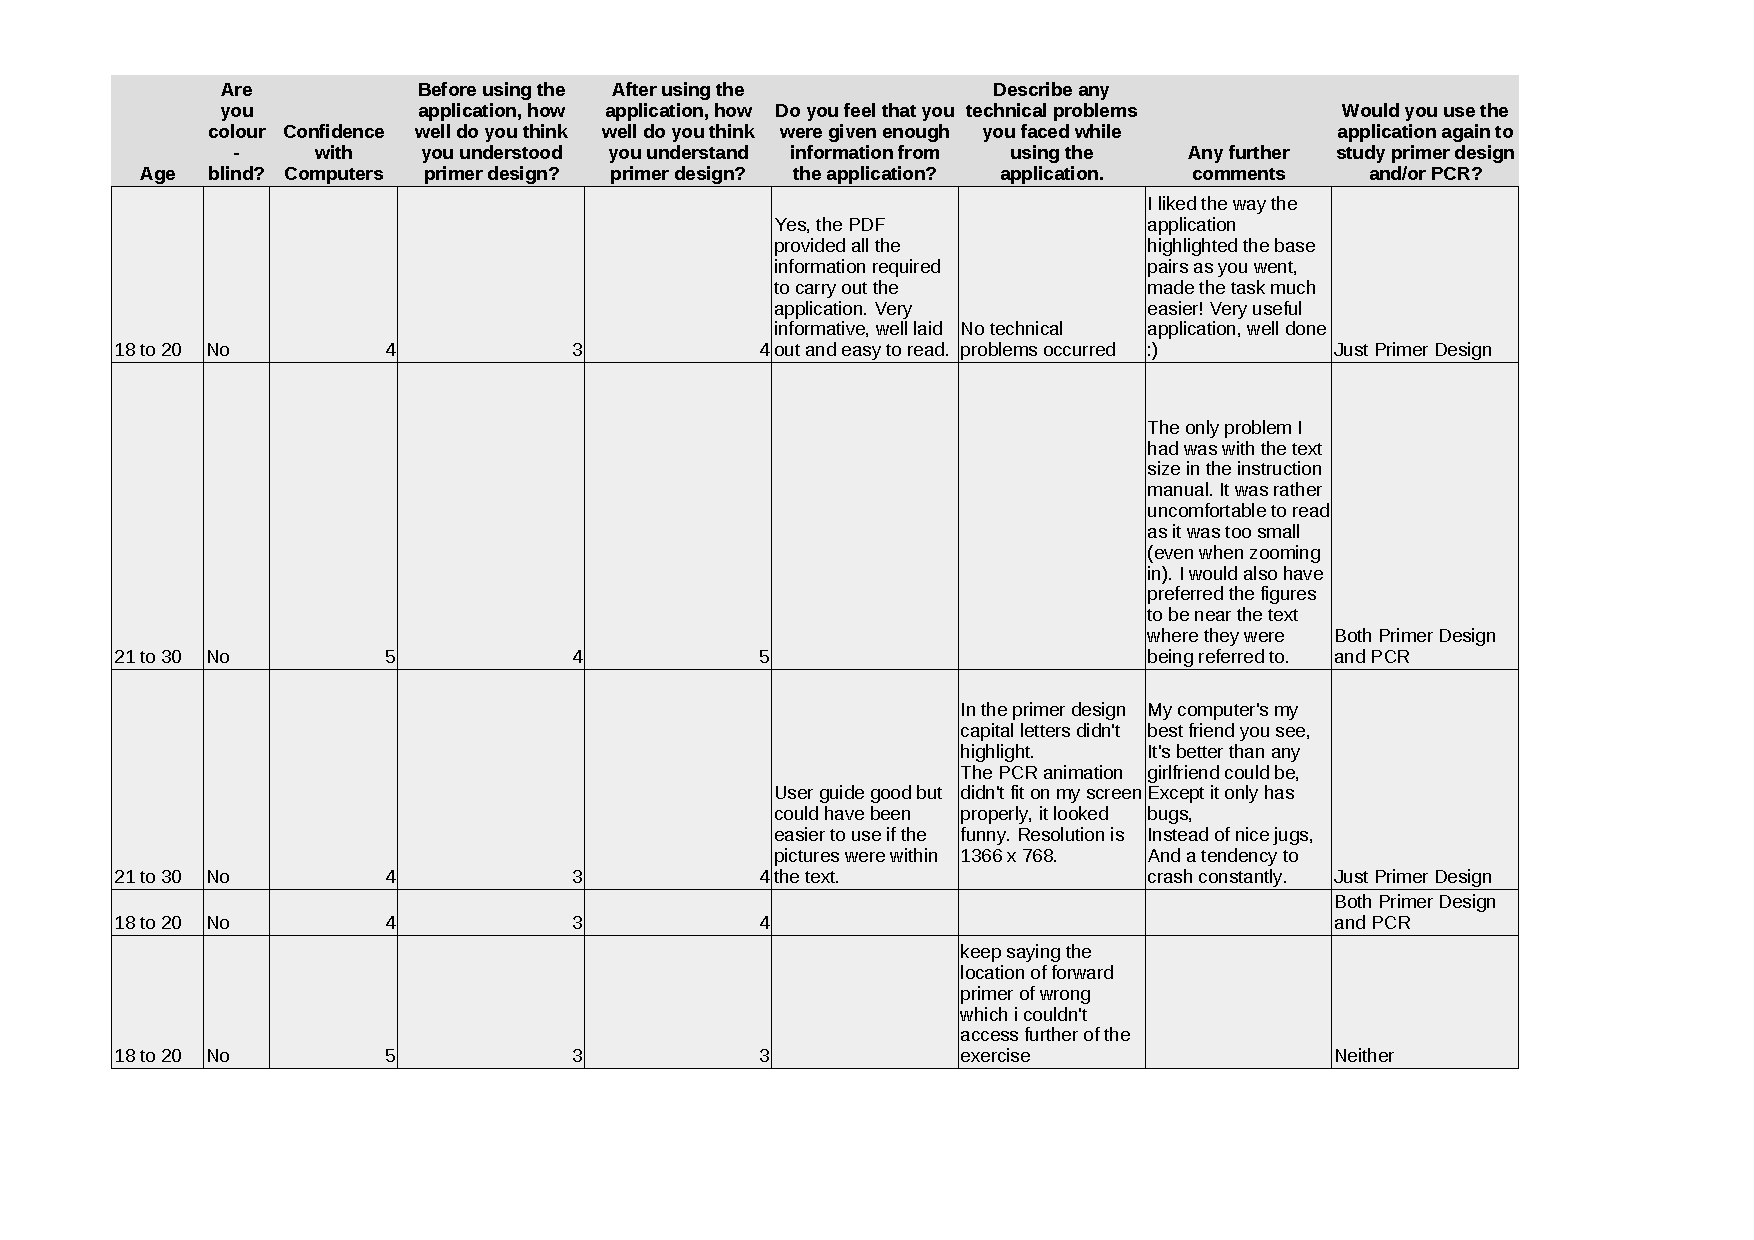
\includepdf[pages=-]{questionnaireResponses.pdf}

\chapter{Current User Guide}
\label{app:userGuideCurrent}
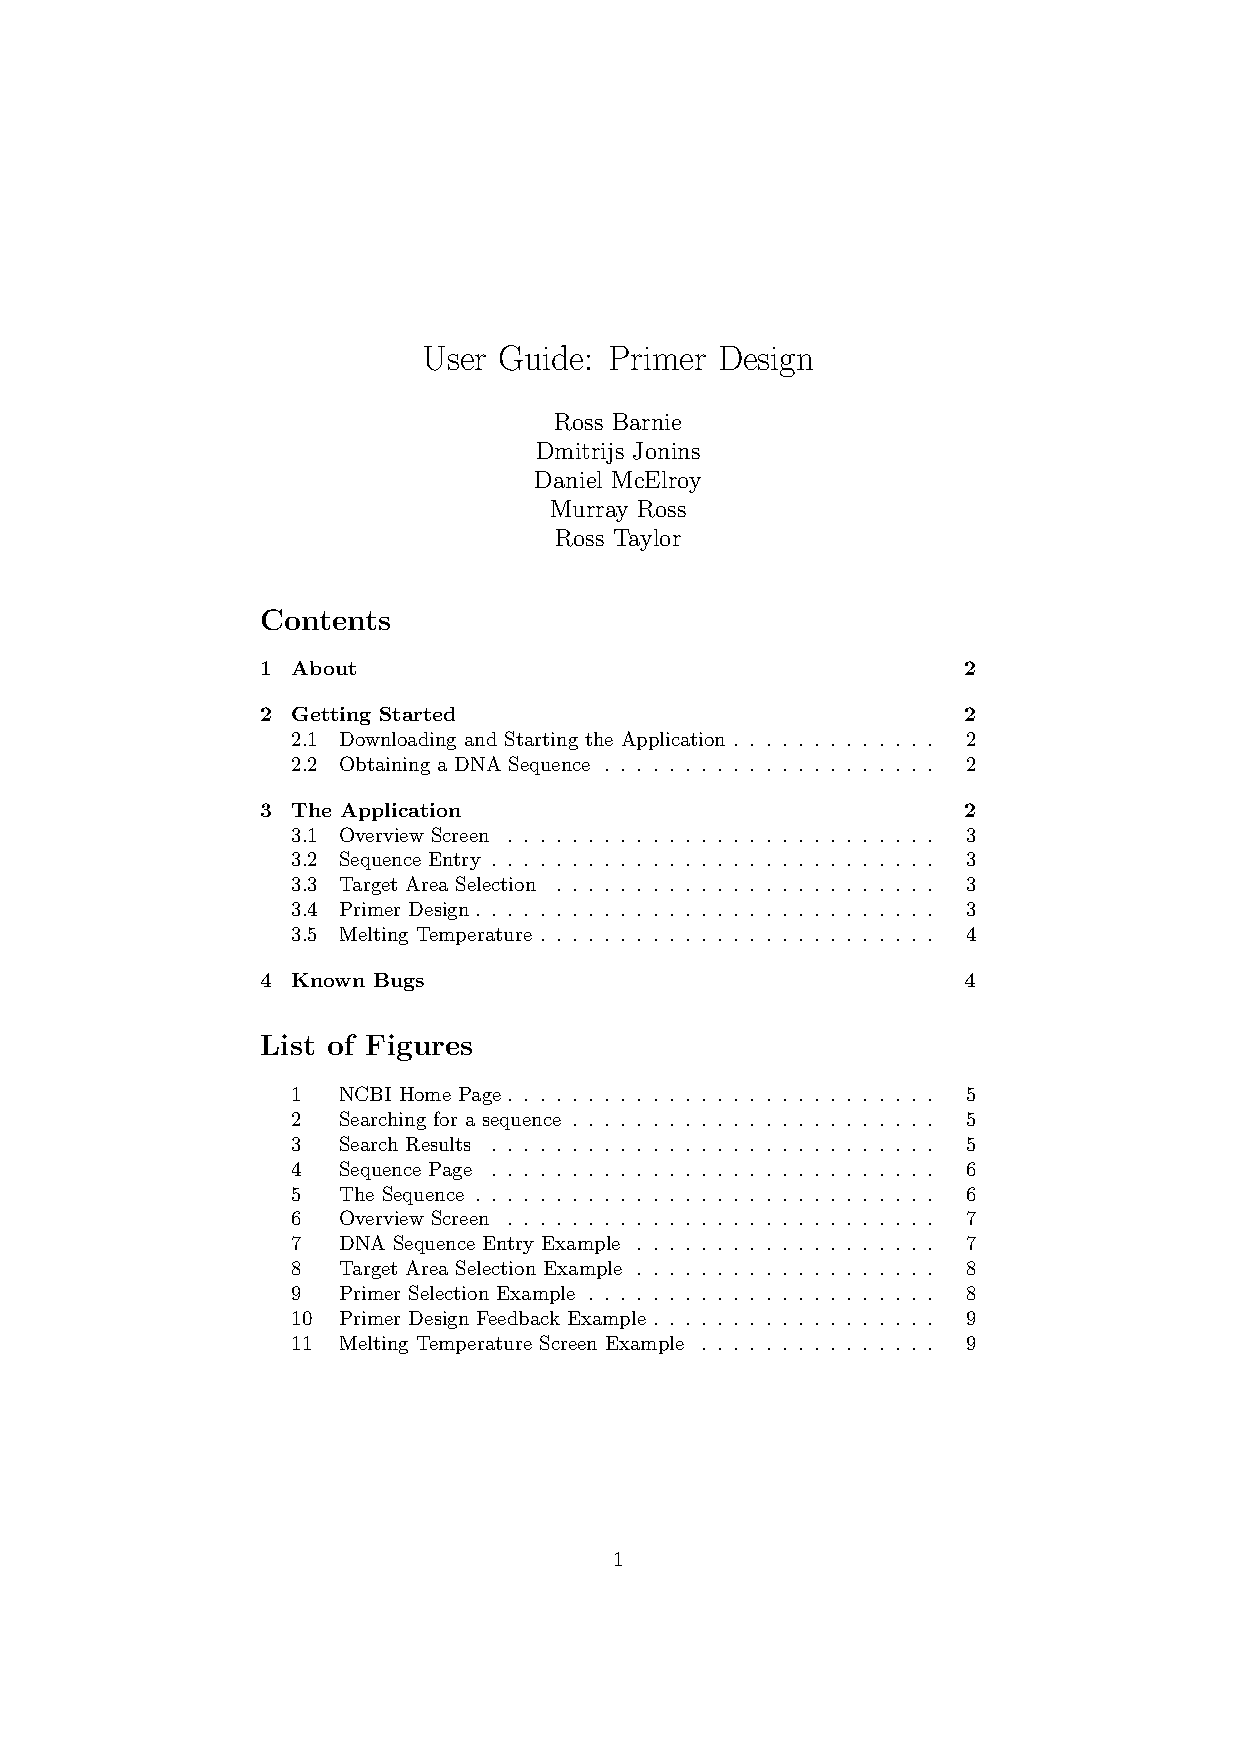
\includepdf[pages=-]{PrimerDesignGuide.pdf}

\clearpage
\bibliographystyle{plain}
\bibliography{references}


\end{document}
